\documentclass[10pt]{article}
\usepackage[verbose, a4paper, hmargin=2.5cm, vmargin=2.5cm]{geometry}

\usepackage{fontspec}
\usepackage{ctex}
\usepackage{paratype}

\usepackage{amsmath}
\usepackage{amssymb}
\usepackage{amsfonts}
\usepackage{esint}
\usepackage{stmaryrd}

\usepackage[mathbf=sym]{unicode-math}
\setmainfont{STIX Two Text}
\setmathfont{STIX Two Math}

\setsansfont{Arial}
\setmonofont{Courier New}

\usepackage{makecell}
\usepackage{wasysym}
\usepackage{pifont}
\usepackage[export]{adjustbox}
\usepackage{graphicx}
\usepackage{mdframed}
\usepackage{booktabs,array,multirow}
\usepackage{tabularx}
\usepackage{hyperref}
\hypersetup{colorlinks=true, linkcolor=blue, filecolor=magenta, urlcolor=cyan,}
\urlstyle{same}
\usepackage[most]{tcolorbox}
\definecolor{mygray}{RGB}{240,240,240}
\tcbset{
  colback=mygray,
  boxrule=0pt,
}
\graphicspath{ {./images/} }
\newcommand{\HRule}{\begin{center}\rule{0.9\linewidth}{0.2mm}\end{center}}
\newcommand{\customfootnote}[1]{
  \let\thefootnote\relax\footnotetext{#1}
}
\newcommand{\lt}{\mathrel{<}}
\newcommand{\gt}{\mathrel{>}}
\newcommand*\circled[1]{\tikz[baseline=(char.base)]{\node[shape=circle,draw,inner sep=1.5pt] (char) {\small #1};}}
\setcounter{MaxMatrixCols}{256}
\begin{document}
Math-Net.Ru

Общероссийский математический портал

С. Н. Аввакумов, Ю. Н. Киселев, М. В. Орлов, Мето- ды решения задач оптимального управления на осно- ве принципа максимума Понтрягина,

Тр. МИАН, 1995, том 211, 3-31

https://www.mathnet.ru/tm1083

Использование Общероссийского математического портала Math-Net.Ru подразумевает, что вы прочитали и согласны с пользовательским согла- шением

https://www.mathnet.ru/rus/agreement

Параметры загрузки:

IP: 109.252.165.210

22 декабря 2025 г., 00:15:55

С.Н. Аввакумов, Ю. Н. Киселев, М. В. Орлов

\section*{Методы решения задач оптимального управления на основе принципа максимума Понтрягина}

\section*{1. Введение}

Применение принципа максимума Понтрягина [1-6] для построения оптималь- ных решений предполагает нахождение сопряженной переменной, участвующей в формулировке принципа максимума. Разработка алгоритмов решения краевой за- дачи принципа максимума представляет самостоятельный интерес и важна для при- ложений. Исследование этих вопросов и в конечном счете создание программ для поиска оптимальных решений определенных классов задач оптимального управле- ния позволяют предоставить в распоряжение инженера программный инструмент для исследования и проектирования управляемых систем. В теории оптимального управления особая роль принадлежит линейной задаче быстродействия, которая рас- сматривается в работах [1-17] и в других книгах и статьях. В теперь уже классиче- ской постановке линейной задачи быстродействия область управления имеет форму компактного выпуклого многогранника, а оптимальное управление при известных условиях является кусочно-постоянной функцией времени со значениями в вершинах многогранника. Наличие точек переключения в экстремальном управлении, связан- ное с формой области управления, сопровождается негладкой в целом зависимостью экстремальной траектории от начального значения сопряженной переменной, что служит одним из источников вычислительной сложности задачи. Поэтому наря- ду с рассмотрением многогранной области управления исследователи обращались к гладким областям управления [18-22]. В работах [21, 22] гладкая область упра- вления описывалась как множество уровня гладкой сильно выпуклой функции f(u) неравенством \(f\left( u\right)  \leq  0\) .

С точки зрения простоты анализа задачи, построения и исследования алгорит- мов решения, их численной реализации более удобным, на наш взгляд, является предложенное в [23] и использованное в [24-35] описание гладкой выпуклой области управления \(U \in  \Gamma \left( {E}^{n}\right)\) в терминах ее опорной функции

\[
c\left( \psi \right)  = \mathop{\max }\limits_{{u \in  U}}\left( {\psi ,u}\right) ,\;\psi  \in  {E}^{n},
\]

подчиненной требованиям гладкости при рф \(\neq\)0 и максимальности ранга матрицы вторых производных с/"(ф). Граница дИ области И параметризуется с помощью градиента ее опорной функции; экстремальное управление и(t, p), отвечающее со- пряженной переменной \(\psi \left( {t,p}\right)\) ,допускает явное аналитическое представление

\[
u\left( {t,p}\right)  = {c}^{\prime }\left( {\psi \left( {t,p}\right) }\right) ,\;p \neq  0, \tag{1.1}
\]

в терминах градиента \({c}^{\prime }\left( \psi \right)\) . Это обстоятельство играет центральную роль в пред- лагаемом подходе, определяет его внешнюю форму и служит основой для конструк- тивного описания методов и алгоритмов решения. Экстремальное управление (1.1) в ходе итерационных процессов решения задачи многократно вычисляется при раз- личных \(t,p\) . В случае \(U = \{ f\left( u\right)  \leq  0\}\) вычисление экстремального управления \(u\left( {t,p}\right)\) представляет в "общей ситуации" вычислительную задачу, трудоемкость которой значительно превышает трудоемкость вычисления экстремального управления по явной формуле (1.1). Использование точного аналитического выражения (1.1) для экстремального управления создает предпосылки для успешного решения задачи, оставляя важную роль применяемому методу.

Для большинства форм областей управления, представляющих интерес для при- ложений, имеются аналитические выражения для опорной функции, могут быть построены в аналитической форме опорные функции гладких аппроксимаций не- гладких областей управления.

Использование свойства выпуклости множеств достижимости линейного упра- вляемого объекта в сочетании с применением аппарата опорных функций позволяет конструктивно описать сведение краевой задачи принципа максимума, содержащей нелинейность \({c}^{\prime }\left( \psi \right)\) ,к задачам Коши. На этом пути осуществляется построение оптимального управления в программной форме; дается описание решения задачи синтеза в гладкой линейной задаче быстродействия [25]: вычисление управляющего сигнала и(x) в данной точке x \(\in\) \({E}^{n} \smallsetminus  \{ 0\}\) сводится к решению задачи Коши для векторного обыкновенного дифференциального уравнения с гладкой правой частью при известном начальном условии. Непрерывным схемам решения отвечают их дис- кретные аналоги.

В разд. 2 обсуждаются затронутые здесь вопросы, относящиеся к задаче быстро- действия: гладкая задача и некоторые методы ее решения; сглаживание области управления, зависимость решения от параметра сглаживания области управления; случай квазилинейной динамики управляемого объекта; приводится пример расчета оптимального решения в трехмерной линейной задаче быстродействия с релейным оптимальным управлением. Расчет проведен с помощью пакета ТАЙМЕР [36].

Применимость подходов и методов, описанных в разд. 2, к другим задачам по- казана в разд. 3 на двух примерах линейных задач. Основное внимание уделяется алгоритмам построения оптимальных решений.

Рассмотрен также пример численного моделирования управления, переводящего линейный объект в начало координат за конечное время. Расчет проведен с помощью пакета КОШИ [37].

\section*{2. Задача быстродействия}

\section*{2.1. Гладкая линейная задача быстродействия}

2.1.1. Постановка задачи. Рассмотрим в \({E}^{n}\) линейную задачу быстролей- ствия с постоянной матрицей \(A\)

\[
\left\{  \begin{array}{ll} \dot{x} = {Ax} + u, & x,u \in  {E}^{n},\;u \in  U,\;U \in  \Gamma \left( {E}^{n}\right) , \\  x\left( 0\right)  = {x}_{0}, & x\left( T\right)  = 0, \\  T \rightarrow  \mathop{\min }\limits_{{u\left( \cdot \right) }}, &  \end{array}\right. \tag{2.1}
\]

Областью управления является гладкий выпуклый компакт U \(\in\) Γ(E \({}^{n}\) ), опреде- ляемый своей опорной функцией

\[
c\left( \psi \right)  = \mathop{\max }\limits_{{u \in  U}}\left( {u,\psi }\right) ,\;\psi  \in  {E}^{n},
\]

достаточно гладкой при \(\psi  \neq  0\) и удовлетворяющей условиям \(c\left( \psi \right)  > 0\) , paнг \({c}^{\prime \prime }\left( \psi \right)  = \; = n - 1\) при \(\parallel \psi \parallel  = 1\) . Начальное состояние \({x}_{0} \neq  0\phi\) азового вектора х принадле- жит области управляемости. Задача (2.1) разрешима в классе гладких допустимых управлений со значениями в U, и единственное оптимальное управление представи- мо в виде (1.1) при некотором \(p = {p}_{\text{ оп }} \neq  0\) :

\[
{u}_{\mathrm{{on}}}\left( t\right)  = u\left( {t,{p}_{\mathrm{{on}}}}\right)  = {c}^{\prime }\left( {\psi \left( {t,{p}_{\mathrm{{on}}}}\right) }\right) ,\;0 \leq  t \leq  {T}_{\mathrm{{on}}}. \tag{2.2}
\]

Здесь \(\psi \left( {t,p}\right)\) — сопряженная переменная, определяемая задачей

\[
\dot{\psi } =  - {A}^{ * }\psi ,{\left. \;\psi \right| }_{t = 0} = p.
\]

Нормированное оптимальное начальное значение роп сопряженной переменной опре- деляется единственным образом. Линейная задача (2.1) сводится к нелинейной кра- евой задаче принципа максимума

\[
\dot{x} = {Ax} + {c}^{\prime }\left( \psi \right) ,\;\dot{\psi } =  - {A}^{ * }\psi ,\;x\left( 0\right)  = {x}_{0},\;x\left( T\right)  = 0,\;0 \leq  t \leq  Т. \tag{2.3}
\]

Задача (2.3) приводится к нелинейной системе конечных уравнений

\[
{x}_{0} - \xi \left( {p,T}\right)  = 0,\;\xi \left( {p,T}\right)  \equiv   - {\int }_{0}^{T}{e}^{-{sA}}{c}^{\prime }\left( {{e}^{-s{A}^{ * }}p}\right) {ds}, \tag{2.4}
\]

\[
N\left( p\right)  = 0, \tag{2.5}
\]

относительно неизвестных \(T > 0,p \in  {E}^{n} \smallsetminus  \{ 0\}\) . Скалярное уравнение (2.5) задает нормировку вектора p, например:

\[
N\left( p\right)  = \parallel p{\parallel }^{2} - 1
\]

\[
N\left( p\right)  = {p}^{ * }{Qp} - 1,
\]

\[
N\left( p\right)  = {p}^{ * }{x}_{0}/\left\lVert {x}_{0} \right\rVert + 1.
\]

Решение системы (2.4), (2.5) может быть получено методом Ньютона, но сходимость имеет место лишь при "достаточно хорошем" нулевом приближении, процедуры по- лучения которого, другие итерационные методы с глобальной сходимостью являют- ся наиболее тонким и содержательным моментом решения задачи (2.1). Обратимся сначала к описанию непрерывной схемы сведения краевой задачи (2.3) к задаче Ко- ши.

2.1.2. Непрерывные схемы проектирования. Схемы проектирования на- чального состояния \({x}_{0}\) на изохрону и точки 0 на множество достижимости описаны в [23-25, 28]. Остановимся только на принципиальных моментах этого подхода. Под проекцией точки \({x}_{0}\) на выпуклый компакт \(Y\) понимается точка \({y}_{0} \in  Y\) ,наименее удаленная от \({x}_{0}\) . Идея элемента наилучшего приближения, восходящая к П.Л. Че- бышеву, в линейной задаче быстродействия привлекалась ранее в работах [16, 15]. Мы используем идею проектирования в гладкой задаче с U \(\in\) Г(Ег’), даем диффе- ренциальное описание конструкции проектирования в динамике, выписывая задачу Коши для опорного вектора \(p\left( T\right)\) , onределяющего проекцию \(\pi \left( T\right)\) точки \({x}_{0}\) на изо- хрону

\[
\sum \left( T\right)  \equiv  \left\{  {\mathbf{x} \in  {E}^{n} : \mathbf{x} = \xi \left( {p,T}\right) ,\parallel p\parallel  = 1}\right\}
\]

в момент времени \(T\) . Кроме того, устанавливается экстремальное свойство вектора \(p\left( T\right)\) как минимизирующей точки гладкой сильно выпуклой по аргументу p функции \(V\left( {p,T}\right) ,0 \leq  T < {T}_{\text{ on }}\) ,которая строится по исходным данным задачи (2.1). Проекция \(\pi \left( T\right) ,0 \leq  T \leq  {T}_{\text{ on }}\) ,допускает представление

\[
\pi \left( T\right)  = \xi \left( {p\left( T\right) ,T}\right) ,\;\parallel p\left( T\right) \parallel  = 1,
\]

причем единичный вектор \(p\left( T\right)\) является внутренней нормалью к изохроне \(\sum \left( T\right)\) в точке \(\pi \left( T\right)  \in  \sum \left( T\right)\) . При фиксированном \(T \in  \left[  {0,{T}_{\text{ on }}}\right)\) вектор \(p\left( T\right)\) определяется конечным уравнением

\[
p + \left[  {{x}_{0} - \xi \left( {p,T}\right) }\right]  /\left\lVert {{x}_{0} - \xi \left( {p,T}\right) } \right\rVert = 0. \tag{2.6}
\]

Конструкция проектирования в динамике приводит к дифференциальному описанию вектора \(p\left( T\right)\) и расстояния \(r\left( T\right)  = \left\lVert {{x}_{0} - \pi \left( T\right) } \right\rVert\) от \({x}_{0}\) до изохроны с помощью задачи Коши

\[
\left\{  \begin{array}{l} \frac{dp}{dT} =  - {\left( rE - \frac{\partial \xi \left( {p,T}\right) }{\partial p} + p{p}^{ * }\right) }^{-1}\left( {E - p{p}^{ * }}\right) \frac{\partial \xi \left( {p,T}\right) }{\partial T}, \\  \frac{dr}{dT} =  - c\left( {{e}^{-T{A}^{ * }}p}\right) , \\  p\left( 0\right)  =  - {x}_{0}/\left\lVert {x}_{0} \right\rVert, \\  r\left( 0\right)  = \left\lVert {x}_{0} \right\rVert,\;0 \leq  T \leq  {T}_{0}, \end{array}\right. \tag{2.7}
\]

которая решается при \(T \geq  0\) до момента \({T}_{0} > 0\) обращения в нуль расстояния \(r\left( T\right)\) ,монотонно убывающего с ростом \(T\) . Существование корня \({T}_{0}\) равносильно разрешимости задачи (2.1). Если р = р(T), r = r(T) — решение задачи (2.7), то оптимальное время \({T}_{\text{ оп }} = {T}_{0}\) , а оптимальное начальное значение сопряженной переменной \({p}_{\text{ on }} = p\left( {T}_{0}\right)\) . Вместо задачи (2.7),имеющей размерность \(n + 1\) ,можно решать задачу размерности n

\[
\left\{  \begin{array}{l} \frac{dp}{dT} =  - {\left( \left\lVert {x}_{0} - \xi \left( p,T\right) \right\rVert E - \frac{\partial \xi \left( {p,T}\right) }{\partial p} + p{p}^{ * }\right) }^{-1}\left( {E - p{p}^{ * }}\right) \frac{\partial \xi \left( {p,T}\right) }{\partial T}, \\  p\left( 0\right)  =  - {x}_{0}/\left\lVert {x}_{0} \right\rVert,\;0 \leq  T \leq  {T}_{0}. \end{array}\right. \tag{2.8}
\]

В (2.7),(2.8) \(E\) — единичная матрица порядка n. Конечное уравнение (2.6) равно- сильно уравнению, имеющему градиентную форму,

\[
{V}_{p}^{\prime }\left( {p,T}\right)  \equiv  p + \left[  {{x}_{0} - \xi \left( {p,T}\right) }\right]  /\Phi \left( {p,T}\right)  = 0,\;p \in  K\left( T\right) , \tag{2.9}
\]

где

\[
\Phi \left( {p,T}\right)  = {p}^{ * }\left[  {{x}_{0} - \xi \left( {p,T}\right) }\right]   \equiv  {p}^{ * }{x}_{0} + {\int }_{0}^{T}c\left( {{e}^{-s{A}^{ * }}p}\right) {ds},
\]

\[
K\left( T\right)  = \left\{  {p \in  {E}^{n} : \Phi \left( {p,T}\right)  < 0}\right\}   \neq  \varnothing \;\text{ п ри }\;0 \leq  T < {T}_{\mathrm{{on}}},
\]

a потенциал \(V\left( {p,T}\right)\) имеет вид

\[
V\left( {p,T}\right)  = \parallel p{\parallel }^{2}/2 - \ln \left[  {-\Phi \left( {p,T}\right) }\right]  ,\;p \in  K\left( T\right) ,\;0 \leq  T < {T}_{\mathrm{{on}}}, \tag{2.10}
\]

и является гладкой сильно выпуклой функцией по первому аргументу в открытом конусе \(K\left( T\right)\) . Вектор \(p\left( T\right)\) , onpeдeляемый задачей Коши (2.8), oбладает экстремаль- ным свойством

\[
V\left( {p\left( T\right) ,T}\right)  = \mathop{\min }\limits_{{\bar{p} \in  K\left( T\right) }}V\left( {\bar{p},T}\right) \;\forall T \in  \left[  {0,{T}_{\mathrm{{on}}}}\right) ,\;p\left( T\right)  = \mathop{\operatorname{argmin}}\limits_{{\bar{p} \in  K\left( T\right) }}V\left( {\bar{p},T}\right) . \tag{2.11}
\]

Сочетание дифференциального описания (2.8) и экстремального описания (2.11) век- тора р(Т) допускает гибкую организацию вычислительного процесса решения зада- чи (2.1) вплоть до полного исключения из вычислительного процесса задачи Коши. Полученное при изучении гладкого случая экстремальное свойство (2.11) сохраняет силу и в негладкой задаче быстродействия. Недостатком потенциала (2.10) являет- ся то, что он определен лишь при \(0 \leq  T < {T}_{\mathrm{{on}}}\) ,на точном решении \({p}_{\mathrm{{on}}},{T}_{\mathrm{{on}}}\) имеет особенность, конус \(K\left( T\right)\) при \(T \rightarrow  {T}_{\mathrm{{on}}} - 0\) cyжается, приближаясь к лучу L = \(\left\{  {\lambda {p}_{\mathrm{{on}}}}\right.\) ,

\[
\lambda  > 0\} \text{ . }
\]

Заметим, что задача Коши (2.7) с симметричной положительно определенной обращаемой матрицей не имеет особенностей при всех T \(\in\) [0, \({T}_{\text{ оп }}\) ]. Аналогичные построения и выводы допускает схема проектирования точки 0 на множество дости- жимости, в которой параметризация сопряженной переменной производится векто- ром \(q = {\left. \psi \right| }_{t = T}\) . Указанный недостаток потенциала (2.10), cssзанный с применяемой reometрической конструкцией проектирования точки х, на изохрону \(\sum \left( T\right)\) , привел к рассмотрению другой геометрической конструкции для решения задачи быстро- действия (2.1) и введению другого потенциала \(F\left( {\eta ,T}\right)\) ,который определен при всех \(T > 0\) . В последней геометрической конструкции вместо проекции \(\pi \left( T\right)\) использует- ся точка \(\widehat{\pi }\left( T\right)\) пересечения изохроны \(\sum \left( T\right)\) с лучом \(L = \left\{  {\lambda {x}_{0},\lambda  \geq  0}\right\}\) , cm. n. 2.1.3 и [26].

2.1.3. Решение задачи быстродействия (2.1) методом потенциалов при специальной параметризации начального значения сопряженной перемен- ной. Пользуясь свободой выбора нормировки начального значения сопряженной пе- ременной, положим

\[
p = \widehat{p}\left( \eta \right)  \equiv  {g}_{0} + {g}_{1}{\eta }_{1} + \ldots  + {g}_{n - 1}{\eta }_{n - 1} \equiv  {g}_{0} + {G\eta }, \tag{2.12}
\]

где \(\eta  = \left( {{\eta }_{1},\ldots ,{\eta }_{n - 1}}\right)  \in  {E}^{n - 1};{g}_{0} =  - {x}_{0}/\left\lVert {x}_{0} \right\rVert;{g}_{1},\ldots ,{g}_{n - 1}\) - opтонормированный базис в \({E}^{n};G = \left( {{g}_{1}\left| \ldots \right| {g}_{n - 1}}\right)  - n \times  \left( {n - 1}\right)\) -матрица. Представление вектора р в форме (2.12) равносильно линейному условию нормировки

\[
N\left( p\right)  \equiv  {p}^{ * }\frac{{x}_{0}}{\left\lVert {x}_{0} \right\rVert} + 1 = 0, \tag{2.13}
\]

которое несущественно отличается от применяемого в методе моментов [7] условия \({p}^{ * }{x}_{0} =  - 1\) . Paзрешение условия (2.13) в форме (2.12) со свободной переменной \(\eta  \in  {E}^{n - 1}\) оказывается чрезвычайно удобным для решения системы уравнений (2.4), (2.13), которая с учетом (2.12) приводится к одному векторному уравнению

\[
{x}_{0} - \xi \left( {\widehat{p}\left( \eta \right) ,T}\right)  = 0 \tag{2.14}
\]

относительно \(\eta  \in  {E}^{n - 1},T > 0\) . Уравнение (2.14) преобразуется к равносильной системе

\[
F\left( {\eta ,T}\right)  = 0, \tag{2.15a}
\]

\[
{F}_{\eta }^{\prime }\left( {\eta ,T}\right)  = 0, \tag{2.156}
\]

где первое уравнение скалярное, а второе (векторное) имеет градиентную форму с потенциалом

\[
F\left( {\eta ,T}\right)  =  - \left\lVert {x}_{0} \right\rVert + {\int }_{0}^{T}c\left( {{e}^{-s{A}^{ * }}\widehat{p}\left( \eta \right) }\right) {ds}. \tag{2.16}
\]

Для получения системы (2.15) уравнение (2.14) умножается скалярно на векторы \(\widehat{p}\left( \eta \right) ,{g}_{1},\ldots ,{g}_{n - 1}\) , oбразующиe базис в \({E}^{n}\) :

\[
\widehat{p}{\left( \eta \right) }^{ * }\left[  {{x}_{0} - \xi \left( {\widehat{p}\left( \eta \right) ,T}\right) }\right]   = F\left( {\eta ,T}\right)
\]

\[
{g}_{j}^{ * }\left[  {{x}_{0} - \xi \left( {\widehat{p}\left( \eta \right) ,T}\right) }\right]   = {F}_{{\eta }_{j}}^{\prime }\left( {\eta ,T}\right) ,\;j = 1,\ldots ,n - 1.
\]

Потенциал (2.16) монотонно возрастает по второму аргументу Т, а при фиксиро- ванном \(T > 0\) является гладкой выпуклой функцией первого аргумента η \(\in\) \({E}^{n - 1}\) с положительно определенной матрицей вторых производных

\[
{F}_{\eta \eta }^{\prime \prime }\left( {\eta ,T}\right)  = {\left. {\int }_{0}^{T}{G}^{ * }{e}^{-{sA}}{c}^{\prime \prime }\left( {e}^{-s{A}^{ * }}p\right) {e}^{-s{A}^{ * }}Gds\right| }_{p = \widehat{p}\left( \eta \right) },
\]

причем

\[
F\left( {\eta ,T}\right)  \rightarrow   + \infty \text{ при }\parallel \eta \parallel  \rightarrow  \infty ,\;T > 0.
\]

Сведение задачи быстродействия (2.1) к системе нелинейных уравнений (2.15) специ- альной структуры является важным техническим этапом решения. Система (2.15) удобна как при качественном анализе, так и при конструировании алгоритмов по- иска ее решения. Для любого \(T > 0\) уравнение (2.156) имеет единственное решение \(\eta  = \widetilde{\eta }\left( T\right) ,\) причем

\[
\widetilde{\eta }\left( T\right)  = \mathop{\operatorname{argmin}}\limits_{{\eta  \in  {E}^{n - 1}}}F\left( {\eta ,T}\right) . \tag{2.17}
\]

При любом \(\eta  \in  {E}^{n - 1}\) уравнение (2.15a) имеет единственный положительный корень \(T = \widetilde{T}\left( \eta \right)\) . Подстановка (2.17) в уравнение (2.15a) приводит к скалярному уравнению

\[
\widetilde{f}\left( T\right)  \equiv  F\left( {\widetilde{\eta }\left( T\right) ,T}\right)  = 0, \tag{2.18}
\]

имеющему единственный положительный корень \({T}_{0}\) . Тогда \({T}_{\mathrm{{on}}} = {T}_{0},{p}_{\mathrm{{on}}} = \widehat{p}\left( {\eta }_{\mathrm{{on}}}\right)\) , \({\eta }_{\text{ on }} \equiv  \widetilde{\eta }\left( {T}_{0}\right)\) — оптимальные параметры, решающие задачу быстродействия (2.1). Итерационный процесс

\[
{\eta }_{0} = 0,\;{T}_{0} = \widetilde{T}\left( {\eta }_{0}\right) ,\;{\eta }_{k + 1} = \widetilde{\eta }\left( {T}_{k}\right) ,\;{T}_{k + 1} = \widetilde{T}\left( {\eta }_{k + 1}\right) ,\;k = 0,1,2,\ldots \tag{2.19}
\]

при \(k \rightarrow  \infty\) cxoglutrca к оптимальной паре ( \({\eta }_{\mathrm{{on}}},{T}_{\mathrm{{on}}}\) ) с квадратичной скоростью [26]. На каждом шаге итерационного процесса (2.19) требуется решать гладкую выпук- лую задачу минимизации потенциала \(F\left( {\eta ,{T}_{k}}\right)  \rightarrow  \min ,\eta  \in  {E}^{n - 1}\) ,и задачу вычисле ния корня \(T = \widetilde{T}\left( {\eta }_{k + 1}\right)\) скалярного уравнения.

Геометрическая интерпретация метода потенциалов в фазовом пространстве и в пространстве (F, η), обоснование квадратичной скорости сходимости процесса (2.19) содержится в [26].

Предложенная схема решения задачи (2.1) эффективна в вычислительном пла- не \(\left[  {{26},{27}}\right]\) и включена в пакеты ТАЙМЕР, TAXIOH,ПОНТРЯГИН.

Рассмотренный подход, разработанный для случая гладких областей управле- ния, применим и в негладком случае, когда нельзя всегда гарантировать единствен- ность минимизирующей точки (2.17) потенциала (2.16). Процедуры сглаживания области управления при этом можно рассматривать как некоторую регуляризацию задачи минимизации потенциала \(F\left( {\eta ,T}\right)  \rightarrow  \min ,\eta  \in  {E}^{n - 1}\) . Данный метод при решении негладких задач хорошо выдерживает введение в задачу малого параме- тра сглаживания области управления благодаря выпуклой структуре потенциала. Потенциал \(F\) содержит всю информацию о решаемой задаче (2.1), имеет хорошо организованную форму, вычислительный процесс описывается в терминах функции \(F\) и ее производных. По-видимому, конструкция потенциала \(F\) будет полезной в задачах, решаемых методом моментов.

2.1.4. Другие постановки задачи быстродействия. В задаче (2.1) концы траектории фиксированы. Используемые подходы применимы для краевых условий вида \(x\left( 0\right)  \in  {M}_{0},x\left( T\right)  \in  {M}_{1}\) ,где \({M}_{0},{M}_{1}\) - множества в \({E}^{n}\) . B [35] рассмотрен слу- чай, korда начальное и конечное множества \({M}_{i},i = 1,2\) ,имеют вид \({M}_{i} = {x}_{i} + {\bar{M}}_{i}\) , где \({\dot{x}}_{i} \in  {E}^{n}\) - точка, \({\bar{M}}_{i} \in  \Gamma \left( {E}^{n}\right)\) - гладкий выпуклый компакт. В [34] рассмотрен случай, когда \({M}_{0} = \left\{  {x}_{0}\right\}\) — одноточечное множество, \({M}_{1}\) — подпространство, а диф- ференциальное уравнение управляемого движения записано в виде \(\dot{x} = {Ax} + \varphi \left( t\right)  + u\) , где \(\varphi \left( t\right)\) — известная функция времени. Отметим, что рассмотренные методы при- менимы для задачи быстродействия в следующей постановке: пусть \(W\left( t\right)\) — непре- рывно зависящий от времени выпуклый компакт в \({E}^{n},z\left( t\right)\) — заданная \(n\) -мерная непрерывная функция времени; \(z\left( 0\right)  \cap  W\left( 0\right)  = \varnothing\) . Tpeбyercя найти первый момент времени \(t = {t}_{1} > 0\) ,когда \(z\left( t\right)  \in  W\left( t\right)\) . Такая постановка задачи быстродействия возникает в теории линейных дифференциальных игр [2], где \(W\left( t\right)\) — альтерниро- ванный интеграл.

\section*{2.2. Процедуры сглаживания выпуклых множеств}

Процедуры сглаживания негладких областей управления позволяют применять методы решения гладких задач для приближенного решения задач с негладкими областями управления.

Теорема 2.1. Для любого выпуклого компакта U0 из Е" и любого числа \(\varepsilon  > 0\) cylцествует выпуклый компакт \({U}_{\varepsilon }\) с расстоянием Хаусдорфа h(0, U, E) \(\leq  \varepsilon\) , причем опорная функция \(c\left( \psi \right)\) компакта UE является гладкой при ψ \(\in\) \({E}^{n} \smallsetminus  \{ 0\} u\) ранг матрицы \({c}^{\prime \prime }\left( \psi \right)\) равен \(n - 1\) .

Для вычислительных приложений особую роль играет конструктивное описание опорной функции сглаженного множества. В основе процедуры сглаживания лежит теорема 2.2, прообразом которой является формула

\[
\max \left( {{c}_{1},{c}_{2}}\right)  = \frac{{c}_{1} + {c}_{2}}{2} + \frac{\left| {c}_{1} - {c}_{2}\right| }{2}.
\]

T e o p e m а 2.2. Пусть \({F}_{1},{F}_{2}\) - два непустых выпуклых компакта в E", опорные функции \({c}_{1}\left( \psi \right) ,{c}_{2}\left( \psi \right)\) которых являются гладкими в \({E}^{n} \smallsetminus  \{ 0\}\) . При любом \(\varepsilon  \geq  0\) функция

\[
c\left( \psi \right)  = \frac{{c}_{1}\left( \psi \right)  + {c}_{2}\left( \psi \right) }{2} + {\left( {\varepsilon }^{2}\parallel \psi {\parallel }^{2} + {\left( \frac{{c}_{1}\left( \psi \right)  - {c}_{2}\left( \psi \right) }{2}\right) }^{2}\right) }^{1/2} \tag{2.20}
\]

является опорной функцией выпуклого компакта

\[
{G}_{\varepsilon } = \left\{  {x \in  {E}^{n} : \left( {x,\psi }\right)  \leq  c\left( \psi \right) ,\psi  \in  {E}^{n}}\right\}  ,
\]

причем \({G}_{0} = \operatorname{conv}\left\{  {{F}_{1},{F}_{2}}\right\}\) . При \(\varepsilon  > 0\) функция (2.20) является гладкой в \({E}^{n} \smallsetminus  \{ 0\}\) , там же ранг с"(ψ) = n-1; G ⊂ int \({G}_{\varepsilon }\) u

\[
0 < h\left( {{G}_{0},{G}_{\varepsilon }}\right)  \leq  \varepsilon \tag{2.21}
\]

Пример 2.1. Пусть \({F}_{1} = \left\{  {x \in  {E}^{n} : \parallel x\parallel  \leq  1}\right\}\) — единичный шар в \({E}^{n},{F}_{2} = \; = \{ v\}\) — одноточечное множество, \(\parallel v\parallel  > 1\) . Множество \({G}_{0} = \operatorname{conv}\left\{  {{F}_{1},{F}_{2}}\right\}\) напоми- нает конус с вершиной \(v\) , ocнованием которого служит шар \({F}_{1}\) . Негладкий выпуклый компакт \({G}_{0}\) аппроксимируется гладким \({G}_{\varepsilon } \in  \Gamma \left( {E}^{n}\right) ,\varepsilon  > 0\) , с опорной функцией

\[
c\left( \psi \right)  = \frac{\parallel \psi \parallel  + \left( {\psi ,v}\right) }{2} + {\left( {\varepsilon }^{2}\parallel \psi {\parallel }^{2} + {\left( \frac{\parallel \psi \parallel  - \left( {\psi ,v}\right) }{2}\right) }^{2}\right) }^{1/2},
\]

c оценкой отклонения (2.21).

Пр и м е р 2.2. Гладкая выпуклая аппроксимация треугольника

\[
{G}_{0} = \operatorname{conv}\left\{  {{v}_{1},{v}_{2},{v}_{3}}\right\}
\]

с вершинами \({v}_{1},{v}_{2},{v}_{3} \in  {E}^{n}\) строится при двукратном применении теоремы 2.2. Представив \({G}_{0}\) в виде \({G}_{0} = \operatorname{conv}\left\{  {{F}_{12} \cup  {v}_{3}}\right\}\) ,где \({F}_{12} = \operatorname{conv}\left\{  {{v}_{1},{v}_{2}}\right\}\) , noстроим выпук- лый компакт \({G}_{\varepsilon },\varepsilon  > 0\) , anпроксимирующий \({G}_{0}\) и определяемый опорной функцией

\[
c\left( {{G}_{\varepsilon },\psi }\right)  = \frac{{c}_{12}\left( \psi \right)  + \left( {{v}_{3},\psi }\right) }{2} + {\left( {\varepsilon }^{2}\parallel \psi {\parallel }^{2} + {\left( \frac{{c}_{12}\left( \psi \right)  - \left( {{v}_{3},\psi }\right) }{2}\right) }^{2}\right) }^{1/2},
\]

где

\[
{c}_{12}\left( \psi \right)  = \frac{\left( {{v}_{1},\psi }\right)  + \left( {{v}_{2},\psi }\right) }{2} + {\left( {\varepsilon }^{2}\parallel \psi {\parallel }^{2} + {\left( \frac{\left( {{v}_{1},\psi }\right)  - \left( {{v}_{2},\psi }\right) }{2}\right) }^{2}\right) }^{1/2},
\]

причем \({G}_{0} \subset  \operatorname{int}{G}_{\varepsilon };0 < h\left( {{G}_{0},{G}_{\varepsilon }}\right)  \leq  {2\varepsilon };{G}_{\varepsilon } - {v}_{0} \in  \Gamma \left( {E}^{n}\right) ;{v}_{0} = \left( {{v}_{1} + {v}_{2} + {v}_{3}}\right) /3\) .

3 аме ча ни е 2.1. Рассмотрим выпуклый компактный многогранник \({M}_{0} = \; = \operatorname{conv}\left\{  {{v}_{1},\ldots ,{v}_{N}}\right\}\) с вершинами \({v}_{1},\ldots ,{v}_{N} \in  {E}^{n}\) . Применение процедуры сглажи- вания \(N - 1\) pa3 (в примере 2.2 \(N - 1 = 2\) ) с положительным параметром ε приводит к построению гладкой выпуклой аппроксимации многогранника \({M}_{0}\) выпуклым ком- пактом \({M}_{\varepsilon }\) ,при этом \(0 < h\left( {M,{M}_{\varepsilon }}\right)  \leq  k\left( N\right)  \cdot  \varepsilon ,{M}_{\varepsilon } - {v}_{0} \in  \Gamma \left( {E}^{n}\right)\) ,где величина \(k\left( N\right)\) определяется последовательностью множеств, участвующих в процедуре сглажива- ния, \({\log }_{2}N \leq  k\left( N\right)  \leq  N - 1,{v}_{0} = \left( {{v}_{1} + \ldots  + {v}_{N}}\right) /N\) . При численной реализации про- цедуры сглаживания программируется лишь формула (2.20), а вычисление опорных функций проводится последовательным обращением к запрограммированной проце- дуре.

3 аме ча н и е 2.2. Известно [38], что для любого непустого выпуклого ком- пакта \(K \subset  {E}^{n}\) и любого числа б > 0 существует компактный выпуклый много- гранник \({M}_{0} = \operatorname{conv}\left\{  {{v}_{1},\ldots ,{v}_{N}}\right\}\) с вершинами \({v}_{j} \in  {E}^{n}\) ,для которого \(h\left( {K,{M}_{0}}\right)  \leq  \delta\) . Отсюда в силу замечания 2.1 следует утверждение теоремы 2.1.

Для множеств, представимых в виде алгебраической суммы отрезков

\[
{U}_{0} = {I}_{1} + \ldots  + {I}_{N}
\]

где \({I}_{j} = \left[  {-{b}_{j},{b}_{j}}\right]  ,{b}_{j} \in  {E}^{n}\) , crлаживающее множество \({U}_{\mu }\) строится путем сглажива- ния отрезков \({I}_{j}\) на основе расчетной формулы

\[
c\left( {{I}_{j}\left( \mu \right) ,\psi }\right)  = {\left( {\psi }^{ * }\left[  \mu E + \left( 1 - \mu /{\left\lVert {b}_{j} \right\rVert}^{2}\right) {b}_{j}{b}_{j}^{ * }\right]  \psi \right) }^{1/2}.
\]

Описанная процедура сглаживания многогранника \({M}_{0}\) проста, конструктивна, при- менима при любой размерности n; она использовалась при разработке пакетов ТАЙ- MEP версия 2.0, TAXHOH и других программ.

Рассмотрим еще процедуру сглаживания плоского выпуклого многоугольника \({M}_{0} = \operatorname{conv}\left\{  {{v}_{1},\ldots ,{v}_{N}}\right\}\) с вершинами \({v}_{j} \in  {E}^{2}\) . По вершинам \({v}_{j}\) определяются: длины сторон \({l}_{j} = \left\lVert {{v}_{j + 1} - {v}_{j}} \right\rVert > 0\) ; единичные векторы \({n}_{j}\) внешних нормалей к сторонам \(\left[  {{v}_{j},{v}_{j + 1}}\right]  ,{n}_{j} = \left( {\cos {t}_{j},\sin {t}_{j}}\right) ,j = 1,\ldots ,N,0 \leq  {t}_{1} < \ldots  < {t}_{N} < {2\pi };{v}_{N + 1} \equiv  {v}_{1};\) центр \({v}_{0} = \left( {{v}_{1} + \ldots  + {v}_{N}}\right) /N = \left( {{v}_{01},{v}_{02}}\right)  \in  {M}_{0}\) . Опишем построение опорной функции \(c\left( {\psi ,\mu }\right)\) crлаженного выпуклого компакта \({M}_{\mu }\) , raкого что \({M}_{\mu } - {v}_{0} \in  \Gamma \left( {E}^{2}\right) ,\mu  > 0\) ; \(h\left( {{M}_{0},{M}_{\mu }}\right)  \rightarrow  0,\mu  \rightarrow   + 0\) . Onophas функция \(c\left( {\psi ,\mu }\right)\) onpeдeляется своим сужением на единичную окружность

\[
{c}_{0}\left( {t,\mu }\right)  = {\left. c\left( \psi ,\mu \right) \right| }_{\psi  = \left( {\cos t,\sin t}\right) }.
\]

Поставленная задача решается спомощьо функцин

\[
{c}_{0}\left( {t,\mu }\right)  = {v}_{01}\cos t + {v}_{02}\sin t - \frac{1}{2\pi }{\int }_{0}^{2\pi }\tau \sin {\tau q}\left( {t + \tau ,\mu }\right) {d\tau },
\]

rne

\[
q\left( {t,\mu }\right)  = \mathop{\sum }\limits_{{j = 1}}^{N}{l}_{j}h\left( {t - {t}_{j},\mu }\right)
\]

\[
h\left( {t,\mu }\right)  = \frac{\mu /4}{{\left( \mu  + \left( 1 - \mu \right) {\sin }^{2}\left( t/2\right) \right) }^{3/2}},
\]

\[
{\int }_{0}^{2\pi }h\left( {t,\mu }\right) {dt} \rightarrow  1\;\left( {\mu  \rightarrow   + 0}\right) ,\;{\int }_{0}^{2\pi }h\left( {t,\mu }\right) {e}^{it}{dt} = 0.
\]

Бункция \({c}_{0}\left( {t,\mu }\right)\) является 2π-периодическим решением дифференциального уравне- ния

\[
{\ddot{c}}_{0} + {c}_{0} = q. \tag{2.22}
\]

Правая часть \(q = q\left( {t,\mu }\right)\) уравнения (2.22) зависит от параметров \({l}_{j},{t}_{j}\) многоуголь- ника \({M}_{0}\) .

Другие способы сглаживания в \({E}^{n}\) , удобные для теоретического анализа, указа- ны в [22, 39].

\section*{2.3. Линейная задача быстродействия с возмущенной областью управления. Зависимость решения от параметра сглаживания}

2.3.1. Предварительные замечания. Введение малого параметра в область управления, применяемое в вычислительной практике (см., напр. [14, 23] и др.) для "улучшения" свойств области, приводит к постановке нового класса задач с возмущениями, для которого построены нетривиальные асимптотики. Задачу бы- стродействия (2.1) с компактной выпуклой областью управления \(U = {U}_{\mu } \subset  {E}^{n}\) , зависящей от параметра \(\mu  \in  \left[  {0,{\mu }_{0}}\right]\) ,будем называть задачей \(\left( {P}_{\mu }\right)\) ,задачу \(\left( {P}_{0}\right)\) - невозмущенной задачей.

Теорема 2.3. Пусть 1) задача (Ро) разрешима в классе измеримых упра- влений; 2) \(h\left( {{U}_{0},{U}_{\mu }}\right)  \rightarrow  0,\mu  \rightarrow   + 0;\) 3) \({U}_{0} \subset  {U}_{\mu }\) . Тогда при \(\mu  > 0\) pa3pewu.ma возмущенная задача \(\left( {P}_{\mu }\right)\) с оптимальным временем \({T}_{\mu } \rightarrow  {T}_{0},\mu  \rightarrow   + 0\) .

Условие 3) в теореме 2.3 можно заменить другим, например, таким: \(0 \in  \operatorname{int}{X}_{0}\left( T\right)\) , \({T}_{0} < T < {T}_{0} + \delta ,\delta  > 0\) ,где \({X}_{0}\left( T\right)\) — множество достижимости невозмущенной си- стемы.

Аппроксимация негладкого выпуклого компакта \({U}_{0},0 \in  {U}_{0}\) ,гладким \({U}_{0},0 \in  {U}_{0}\) ,гладким \({U}_{\mu } \in  \Gamma \left( {E}^{n}\right)\) и численное решение гладкой задачи (Ри) дают при малых \(\mathbf{\mu }\) приближение к реше- нию задачи ( \({P}_{0}\) ). Cледует обратить внимание на то, что в гладкой задаче ( \({P}_{\mu }\) ) pe- шение единственно всегда, тогда как в задаче (Ро) оптимальное управление может быть неединственным. Рассмотрение гладких задач как аппарата для аппроксима- ции негладких оправданно при наличии удобных процедур сглаживания негладких областей управления и методов решения гладких задач. Отметим, что, как правило, сглаженная задача \(\left( {P}_{\mu }\right)\) может быть решена только численно, даже в тех отдельных примерах, когда невозмущенная задача проста и ее решение известно, т.е. проце- дуры сглаживания имеют вычислительную направленность. При дополнительных предположениях о задачах \(\left( {P}_{\mu }\right) ,\left( {P}_{0}\right)\) возможно получение более полной информации о связи между их решениями: об асимптотике возмущения решения по параметру μ, о связи оптимальных управлений в этих задачах при малых \(\mu\) . Знание вида асим- птотических разложений позволяет на основе выполненных расчетов для несколь- ких малых значений параметра \({\mu }_{1},\ldots ,{\mu }_{l}\) построить экстраполяционное уточнение решения задачи ( \({P}_{0}\) ).

2.3.2. Гладкая зависимость решения от параметров. Пусть с \(\left( {\psi ,\mu }\right)\) — опорная функция области управления \({U}_{\mu };\mu  \in  \left[  {0,{\mu }_{0}}\right]\) . Оптимальное решение задачи \(\left( {P}_{\mu }\right)\) , onределяемое параметрами

\[
{T}_{\mathrm{{on}}}\left( \mu \right) ,\;{p}_{\mathrm{{on}}}\left( \mu \right) ,\;\left\lVert {{p}_{\mathrm{{on}}}\left( \mu \right) } \right\rVert = 1,\;0 \leq  \mu  \leq  {\mu }_{0}, \tag{2.23}
\]

при определенных условиях гладко зависит от \(\mathbf{\mu }\) ; оптимальное время и начальное значение сопряженной переменной (2.23) гладко зависят от μ и определяются задачей Kowu

\[
\left\{  \begin{array}{ll} \frac{dT}{d\mu } = g\left( {p,T,\mu }\right) , & T\left( {\mu }_{0}\right)  = {T}_{\mathrm{{on}}}\left( {\mu }_{0}\right) , \\  \frac{dp}{d\mu } = G\left( {p,T,\mu }\right) , & p\left( {\mu }_{0}\right)  = {p}_{\mathrm{{on}}}\left( {\mu }_{0}\right) ,\;0 \leq  \mu  \leq  {\mu }_{0}, \end{array}\right. \tag{2.24}
\]

где

\[
g =  - \left( {{p}^{ * }\left( {\partial \xi /\partial \mu }\right) }\right) /\left( {{p}^{ * }\left( {\partial \xi /\partial T}\right) }\right) ,
\]

\[
\xi \left( {p,T,\mu }\right)  =  - {\int }_{0}^{T}{e}^{-{sA}}{c}_{\psi }^{\prime }\left( {{e}^{-s{A}^{ * }}p,\mu }\right) {ds}
\]

\[
G =  - {\left( p{p}^{ * } - \frac{\partial \xi }{\partial p}\right) }^{-1}\left( {E - \frac{\left( {\partial \xi /\partial T}\right) {p}^{ * }}{{p}^{ * }\left( {\partial \xi /\partial T}\right) }}\right) \frac{\partial \xi }{\partial \mu }.
\]

Это возможно в предположении, что \({U}_{\mu } \in  \Gamma \left( {E}^{n}\right) ,\mu  \in  \left[  {0,{\mu }_{0}}\right]\) ,при достаточно гладкой зависимости опорной функции \(c\left( {\psi ,\mu }\right)\) от своих аргументов. Задача (2.24) использо- валась для численного решения задачи ( \({P}_{0}\) ). При малых \(\mu  > 0\) для оптимального времени \(T\left( \mu \right)\) в задаче \(\left( {P}_{\mu }\right)\) имеет место соотношение

\[
T\left( \mu \right)  = T\left( 0\right)  + {T}_{1}\mu  + O\left( {\mu }^{2}\right) ,\;\mu  \rightarrow   + 0, \tag{2.25}
\]

где \({T}_{1}\) — число, от μ не зависящее. Задача (2.24) остается в силе при 0 < μ \(\leq  {\mu }_{0}\) , если условие гладкости нарушается только при \(\mu  = 0\) . При негладком Ио соотно- шение (2.25) с главным членом возмущения, имеющим порядок μ, может оказаться неверным.

2.3.3. Примеры асимптотик по малому параметру сглаживания. Если \({U}_{0}\) — негладкий выпуклый компакт, то для времени Т(μ) возможно представление при \(\mu  \rightarrow   + 0\)

\[
T\left( \mu \right)  = T\left( 0\right)  + \mathop{\sum }\limits_{{k = 1}}^{m}{\mu }^{k}{P}_{k}\left( {\ln \mu }\right)  + o\left( {\mu }^{m}\right)  =
\]

\[
= T\left( 0\right)  + \mu \left[  {{T}_{11}\ln \mu  + {T}_{10}}\right]   + {\mu }^{2}\left[  {{T}_{22}{\ln }^{2}\mu  + {T}_{21}\ln \mu  + {T}_{20}}\right]   + \ldots , \tag{2.26}
\]

где \({P}_{k}\left( s\right)  -\) многочлен степени не больше \(k\) с коэффициентами \({T}_{k\varkappa },0 \leq  \varkappa  \leq  k\) , не зависящими от \(\mu\) . Появление логарифмических членов в (2.26) связано с видом главного члена в интеграле

\[
I\left( \mu \right)  \equiv  {\int }_{0}^{1}{\left( \mu  + {\tau }^{2}\right) }^{-1/2}{d\tau } =  - \frac{1}{2}\ln \mu  + {c}_{0} + {c}_{1}\mu  + \ldots
\]

при малых \(\mu  > 0\) . Разложение (2.26) установлено в ряде модельных примеров, изу- чение которых предшествовало обоснованию многомерных результатов.

B [31] рассмотрена задача \(\left( {P}_{\mu }\right)\)

\[
n = 2,\;A = \left( \begin{array}{ll} 0 & 1 \\  0 & 0 \end{array}\right) ,\;{U}_{\mu } : c\left( {\psi ,\mu }\right)  = \sqrt{\mu {\psi }_{1}^{2} + {\psi }_{2}^{2}}. \tag{2.27}
\]

Здесь в невозмущенной задаче (Ро) (тележка) область управления

\[
{U}_{0} = \left\{  {{u}_{1} = 0,\left| {u}_{2}\right|  \leq  1}\right\}
\]

— отрезок, а возмущенная область управления

\[
{U}_{\mu } = \left\{  {{u}_{1}^{2}/\mu  + {u}_{2}^{2} \leq  1}\right\}   \in  \Gamma \left( {E}^{2}\right)
\]

ограничена эллипсом с полуосями \({\mu }^{1/2},1;\mu  > 0\) . Оптимальное время \(T\left( \mu \right)\) в задаче (2.27) допускает представление (2.26), причем для начальных состояний, не лежа- щих на линии переключения задачи ( \({P}_{0}\) ), \({T}_{11} > 0,\left[  {T\left( \mu \right)  - T\left( 0\right) }\right]  /\mu  \rightarrow  \infty ,\mu  \rightarrow   + 0\) (недифференцируемость \(T\left( \mu \right)\) в нуле). Разложение

\[
T\left( \mu \right)  = T\left( 0\right)  + \mathop{\sum }\limits_{{k = 1}}^{\infty }{\mu }^{k}{P}_{k}\left( {\ln \mu }\right)
\]

сходится при \(0 < \mu  \leq  {\mu }_{0},{\mu }_{0} > 0\) .

B [32] рассмотрен пример сглаживания области управления для математическо- го маятника

\[
n = 2,\;A = \left( \begin{array}{cc} 0 & 1 \\   - 1 & 0 \end{array}\right) ,\;{U}_{\mu } : c\left( {\psi ,\mu }\right)  = \sqrt{\mu {\psi }_{1}^{2} + {\psi }_{2}^{2}}. \tag{2.28}
\]

Анализ примера (2.28) оказался более сложным по сравнению с анализом задачи (2.27), так как в этом случае уравнения принципа максимума не могут быть про- интегрированы в конечном виде. Для "типичных" начальных состояний в (2.28) установлено разложение (2.26).

B [33] рассмотрена задача сглаживания для математического маятника с дву- мерным управлением

\[
n = 2,\;A = \left( \begin{array}{cc} 0 & 1 \\   - 1 & 0 \end{array}\right) ,\;{U}_{\mu } : c\left( {\psi ,\mu }\right)  = \sqrt{\mu {\psi }_{1}^{2} + {\psi }_{2}^{2}} + \sqrt{{\psi }_{1}^{2} + \mu {\psi }_{2}^{2}}.
\]

Здесь \({U}_{0} = \left\{  {\left| {u}_{i}\right|  \leq  1,i = 1,2}\right\}\) — квадрат. Для "типичных" начальных состояний в этой задаче имеет место соотношение (2.26).

Для случая невозмущенной области управления в форме отрезка или алгебраи- ческой суммы конечного числа отрезков С.H. Аввакумовым дано обоснование мно- гомерных аналогов этих результатов; часть из них приведена в п. 2.3.4.

Для задачи ( \({P}_{0}\) )

\[
{\dot{x}}_{1} = {x}_{2} + {u}_{1},\;{\dot{x}}_{2} =  - {x}_{1} + {u}_{2},\;{U}_{0} = \left\{  {\left| {u}_{i}\right|  \leq  1,i = 1,2}\right\}
\]

при вОзмущении области управления вида

\[
{U}_{\varepsilon } = \left\{  {{\left| {u}_{1}\right| }^{p} + {\left| {u}_{2}\right| }^{p} \leq  1}\right\}  ,\;p = 1 + 1/\varepsilon ,\;\varepsilon  \rightarrow   + 0,
\]

имеет место (для "типичных" начальных состояний) степенное разложение опти- мального времени

\[
T\left( \varepsilon \right)  = T\left( 0\right)  + \mathop{\sum }\limits_{{k = 1}}^{\infty }{\varepsilon }^{k}{T}_{k}
\]

сходящееся при малых \(\varepsilon\) . Последний пример рассмотрен Ю. Н. Киселевым и О.H. Ши- мохиной. Многомерные аналоги этого результата исследованы О.H. Шимохиной.

2.3.4. Теорема об асимптотике сглаживания. Рассмотрим в \({E}^{n}\) невозму- щенную линейную задачу быстродействия (2.1) (задачу (P)) с областью управле- ния, имеющей форму отрезка:

\[
{U}_{0} = \left\{  {{u}_{1} = \ldots  = {u}_{n - 1} = 0,\left| {u}_{n}\right|  \leq  1}\right\}  ,
\]

T.e.

\[
{U}_{0} = \left[  {-b,b}\right]  ,\;b = {\left( 0,\ldots ,0,1\right) }^{ * }.
\]

В возмущенной задаче \(\left( {P}_{\mu }\right)\) область управления

\[
{U}_{\mu } = \left\{  {\left( {{u}_{1}^{2} + \ldots  + {u}_{n - 1}^{2}}\right) /\mu  + {u}_{n}^{2} \leq  1}\right\}
\]

имеет форму сжатого эллипсоида и \(h\left( {{U}_{0},{U}_{\mu }}\right)  \rightarrow  0,\mu  \rightarrow   + 0\) . Изучается зависи- мость между решениями задач \(\left( {P}_{\mu }\right)\) и \(\left( {P}_{0}\right)\) при малых \(\mu\) . Предполагается, что \(\det \left( {b,{Ab},\ldots ,{A}^{n - 1}b}\right)  \neq  0\) ; начальное состояние ход допускает разрешимость задачи \(\left( {P}_{0}\right)\) ; пусть (р0, \({T}_{0}\) ) — оптимальная пара в задаче (Ро), ро — нормированное опти- мальное начальное значение сопряженной переменной, \({T}_{0}\) — оптимальное время,

\[
{u}_{0}\left( t\right)  = \operatorname{sgn}\left[  {{b}^{ * }{e}^{-t{A}^{ * }}{p}_{0}}\right]   = \operatorname{sgn}{\psi }_{n}\left( {t,{p}_{0}}\right)
\]

— единственное кусочно-постоянное управление в \(\left( {P}_{0}\right)\) .

Неизвестные оптимальное время \({T}_{\mu }\) и оптимальное начальное значение сопря- женной переменной \({p}_{\mu }\) в задаче \(\left( {P}_{\mu }\right) ,\mu  \geq  0\) , ompeдensitoтся системой уравнений

\[
\xi \left( {p,T,\mu }\right)  - {x}_{0} = 0,\;\parallel p{\parallel }^{2} - 1 = 0 \tag{2.29}
\]

относительно \(p\) и \(T\) . В системе (2.29)

\[
\xi \left( {p,T,\mu }\right)  =  - {\int }_{0}^{T}{e}^{-{sA}}u\left( {s,p,\mu }\right) {ds},\;T > 0,\;p \in  {E}^{n} \smallsetminus  \{ 0\} ,
\]

\[
u\left( {s,p,\mu }\right)  = \mathop{\operatorname{argmax}}\limits_{{v \in  {U}_{\mu }}}\left( {\psi \left( {s,p}\right) ,v}\right) ,\;\psi \left( {s,p}\right)  = {e}^{-s{A}^{ * }}p. \tag{2.30}
\]

B задаче ( \({P}_{\mu }\) ), \(\mu  > 0\) , omтимальное управление существует, единственно, единич- ный вектор \(p = {p}_{\mu }\) , onределяющий в (2.30) оптимальное управление, также является единственным.

Предполагается, что оптимальная пара (ро, то) в задаче (Ро) удовлетворяет усло- виям регулярности (предположения 2.1, 2.2).

\(\Pi\) ре д п о л о ж е н н е 2.1. Все корни функции \({\psi }_{n}\left( {t,{p}_{0}}\right)  \equiv  {b}^{ * }{e}^{-t{A}^{ * }}{p}_{0}\) на от- резке времени \(\left[  {0,{T}_{0}}\right]\) npocтыe и лежат внутри этого отрезка, т.е.

\[
0 < {\theta }_{1} < \ldots  < {\theta }_{N} < {T}_{0};\;{\psi }_{n}\left( {{\theta }_{j},{p}_{0}}\right)  = 0,\;{\dot{\psi }}_{n}\left( {{\theta }_{j},{p}_{0}}\right)  \neq  0,\;j = 1,\ldots ,N.
\]

\(B\) этом случае в окрестности точки (ро,То) \(\in\) \({E}^{n + 1}\) определена и непрерывна матрица \(G\left( {p,T}\right)  = \partial \xi \left( {p,T,0}\right) /\partial p\) , которую можно представить в виде суммы N матриц ранга 1 [23]. Положим \({G}_{0} = G\left( {{p}_{0},{T}_{0}}\right)\) .

Предположение 2.2. Ранг G0 = n -1.

Предположение 2.2 ограничивает снизу число N точек переключения оптималь- ного управления в задаче ( \({P}_{0}\) ): \(N \geq  n - 1\) . В случае матрицы \(A\) ,имеющей только дей- ствительные собственные значения, предположение 2.2 означает, что \(N = n - 1\) . При сделанных предположениях система (2.29) имеет единственное решение р, \({p}_{\mu },{T}_{\mu } > 0\) при \(\mu  \geq  0\) .

Основной результат, на котором основано исследование решения р, но истемы (2.29) при \(\mu  \geq  0\) ,заключается в следующем.

Ут в ер ж д е н и е 2.1. При малых \(\mu  \geq  0,\left\lVert {p - {p}_{0}} \right\rVert,\left| {T - {T}_{0}}\right|\) левая часть си- стемы (2.29) допускает представление

\[
\left( \begin{array}{c} \xi \left( {p,T,\mu }\right)  - {x}_{0} \\  \parallel p{\parallel }^{2} - 1 \end{array}\right)  = \Lambda \left( {p,T,\mu }\right)  + \omega \left( \mu \right) \Pi \left( {p,T,\mu }\right) ,
\]

где \(\omega \left( 0\right)  = 0,\omega \left( \mu \right)  = \mu \ln \mu\) при \(\mu  > 0\) ; векторные функции \(\Lambda\) ,П представимы абсо- лютно и равномерно сходящимися степенными рядами в некоторой окрестности точки \(\left( {{p}_{0},{T}_{0},0}\right)  \in  {E}^{n + 2}\) , причем в этой точке \(\Pi = \Lambda = 0\) , det \(\partial \Lambda /\partial \left( {p,T}\right)  \neq  0\) .

Из утверждения следует

Те о ре м а 2.4. При сделанных предположениях для оптимального времени \({T}_{\mu }\) в задаче \(\left( {P}_{\mu }\right)\) cnpaseдливо представление

\[
{T}_{\mu } = {T}_{0} + \mathop{\sum }\limits_{{k = 1}}^{m}{\mu }^{k}\left[  {\mathop{\sum }\limits_{{x = 1}}^{k}{T}_{kx}{\ln }^{x}\mu }\right]   + o\left( {\mu }^{m}\right) ,\;\mu  \rightarrow   + 0, \tag{2.31}
\]

где \({T}_{0}\) - onmuмальное время в задаче \(\left( {P}_{0}\right) ;m \geq  1\) - натуральное число; \({T}_{kx}\) - коэффициенты, не зависящие от μ.

Аналогичное представление имеет место для \({p}_{\mu }\) .

Бесконечные ряды для \({T}_{\mu }\) и влиясиянные вместо конечного соотношения (2.31) для \({T}_{\mu }\) и \({p}_{\mu }\) ,оказываются сходящимися при \(0 < \mu  \leq  {\mu }_{0}\) для некоторого \({\mu }_{0} > 0\) .

Релейное оптимальное управление и гладким оптимальным управлением и(t, p, μ) задачи (p, при малых и. Именно при любом \(\delta  > 0\)

\[
\left. {\operatorname{mes}\left\{  {t \in  \left[  {0,{T}_{\mu }}\right]   : \left| {u\left( {t,{p}_{\mu },\mu }\right)  - u\left( {t,{p}_{0},0}\right) }\right|  \geq  \delta }\right. }\right\}   \rightarrow  0,\;\mu  \rightarrow   + 0.
\]

Введем множество

\[
{E}_{\gamma } = \left[  {0,{T}_{0}}\right]   \smallsetminus  \mathop{\bigcup }\limits_{{j = 1}}^{N}\left( {{\theta }_{j} - \gamma ,{\theta }_{j} + \gamma }\right) ,\;\gamma  > 0,
\]

полученное выбрасыванием из отрезка \(\left[  {0,{T}_{0}}\right]\) малых окрестностей точек переключе- ния \({\theta }_{j}\) невозмущенной задачи ( \({P}_{0}\) ). При любом \(\gamma  > 0\)

\[
\mathop{\max }\limits_{{t \in  {E}_{\gamma }}}\left| {u\left( {t,{p}_{\mu },\mu }\right)  - u\left( {t,{p}_{0},0}\right) }\right|  \rightarrow  0,\;\mu  \rightarrow   + 0,
\]

т.е. оптимальное управление в задаче (Pμ) сходится к оптимальному управлению задачи \(\left( {P}_{0}\right)\) равномерно на множестве \({E}_{\gamma }\) .

2.4. Примеры расчета оптимального решения

в линейной задаче быстродействия с релейными управлениями.

Графический пакет ТАЙМЕР для решения линейной задачи быстродействия

Рассмотрим задачув \({E}^{3}\)

\[
\left\{  \begin{array}{l} \dot{x} = {Ax} + {bu},\;\left| u\right|  \leq  1, \\  x\left( 0\right)  = {x}_{0},\;x\left( T\right)  = 0, \\  T \rightarrow  \min , \end{array}\right. \tag{2.32}
\]

при

\[
A = \left( \begin{array}{ccc} 0 & 1 & 0 \\  0 & {a}_{22} & {a}_{23} \\  0 & {a}_{32} & {a}_{33} \end{array}\right) ,\;b = \left( \begin{array}{l} 0 \\  0 \\  1 \end{array}\right) ,\;{x}_{0} = \left( \begin{array}{l} {x}_{01} \\  {x}_{02} \\  {x}_{03} \end{array}\right) . \tag{2.33}
\]

В расчете положено

\[
{a}_{22} = {a}_{33} =  - 0,1;\;{a}_{23} =  - {a}_{32} = 3;\;{x}_{01} = {x}_{02} = 2,\;{x}_{03} = 0. \tag{2.34}
\]

Этот пример моделирует следующую ситуацию. Рассмотрим вращение тяжелого вала с моментом инерции \(J\) без трения под действием вращательного момента M, описываемое уравнением

\[
J\ddot{\theta } = M,\;\theta \left( 0\right)  = {\theta }_{0},\;\dot{\theta }\left( 0\right)  = {\theta }_{1},\;\theta \left( T\right)  = \dot{\theta }\left( T\right)  = 0,
\]

где θ — угловое перемещение вала. Если считать управлением ограниченный по модулю момент \(M\) , то эта задача быстродействия \(T \rightarrow  \min\) совпадает с задачей для тележки [1, пример 1]. Если момент М создается электромотором, то можно считать, что

\[
M =  - {k}_{1}\dot{\theta } + {k}_{2}I,
\]

где ток I описывается линейным уравнением

\[
L\dot{I} + {RI} + {k}_{3}\dot{\theta } = {k}_{4}u,
\]

в котором управление и подчинено ограничению \(\left| u\right|  \leq  1\) и характеризует напря- жение \(\left( {L,R,{k}_{j} - }\right.\) известные положительные числа). Введение фазовых координат \({x}_{1} = \theta ,{x}_{2} = \dot{\theta },{x}_{3} = I\) приводит к системе (2.32),(2.33). В случае (2.34) матрица \(A\) имеет собственные значения 0, \(- 0,1 \pm  {3i}\) . Herладкая задача (2.32)-(2.34) имеет релейное оптимальное управление. Ее решение проведено на IBM PC с помощью пакета TAЙMEP версия 2.0 при параметре сглаживания \(\mu  = {10}^{-6}\) (малые полуоси сильно сжатого эллипсоида, аппроксимирующего отрезок [—6, b], равны 10—3). Вы- численное оптимальное время \({T}_{on} \approx  7,{6771}\) , onтимальное управление имеет четыре точки переключения \({\tau }_{1} \approx  4,{63},{\tau }_{2} \approx  4,{94},{\tau }_{3} \approx  6,{63},{\tau }_{4} \approx  7,{13}\) . Ha рис. 1 изо- бражены графики оптимального управления и координат оптимальной траектории. Полученный график оптимального управления визуально неотличим от релейного. Точное оптимальное управление имеет вид

\[
u\left( t\right)  = \operatorname{sgn}{\psi }_{3}\left( t\right) ,\;{\psi }_{3}\left( t\right)  = {c}_{1} + {e}^{-0,{1t}}\left( {{c}_{2}\cos {3t} + {c}_{3}\sin {3t}}\right)
\]

\begin{center}
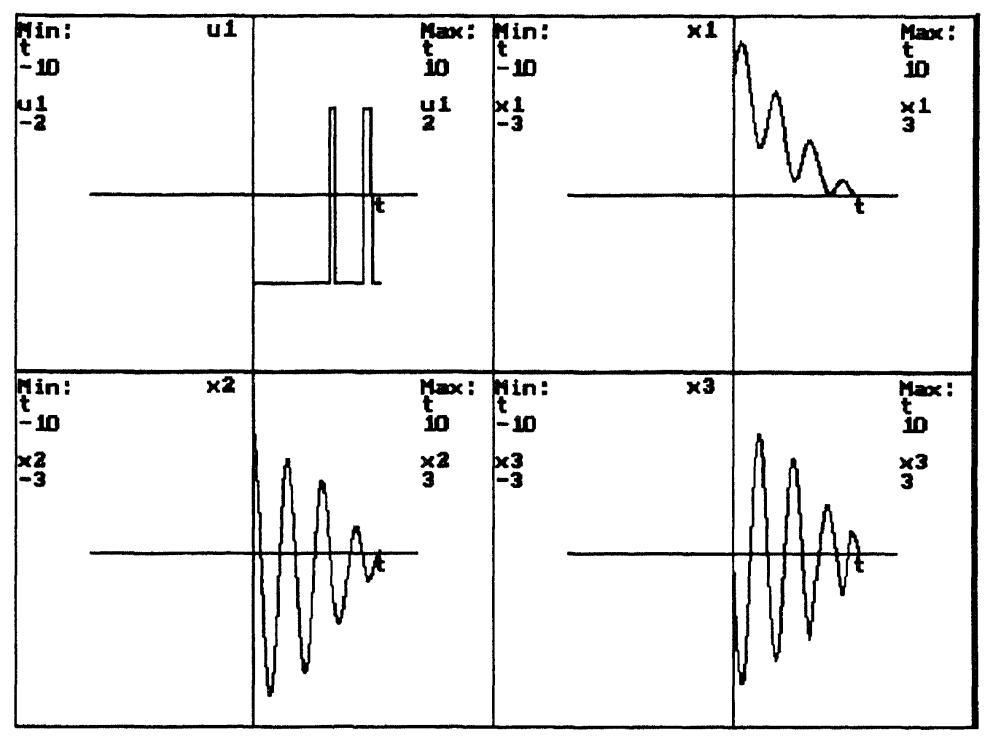
\includegraphics[max width=0.9\textwidth]{images/bo_d54811f7aajc73fuvcmg_17_264_72_988_739_0.jpg}
\end{center}
\hspace*{3em} 

Prac. 1

при некоторых постоянных \({c}_{1},{c}_{2},{c}_{3}\) ,связанных определенным образом с начальными значениями \({p}_{i} = {\psi }_{i}\left( 0\right) ,i = 1,2,3\) , conряженной переменной. Программа осуществля- ет вычисление параметров \({p}_{i}\) и оптимального времени.

Пакеты ТАЙМЕР версия 1.0 и 2.0 [36, 40] предназначены для численного ис- следования линейных задач быстродействия. В них реализован широкий набор сер- висных функций (см. подразд. 3.3, сервисные функции пакета КОШИ), что делает пакеты удобным инструментом для научных и инженерных исследований. Пакеты позволяют исследовать поведение оптимальных управлений и траекторий. В ка- ждой из версий реализовано по четыре численных метода решения линейной задачи быстродействия, имеется возможность перехода с одного метода на другой в процес- се расчета. По окончании расчета пользователь может посмотреть получившиеся значения оптимального времени, начальных значений сопряженной переменной, по- лучить графическую и цифровую информацию об оптимальном решении. Матрица системы может иметь собственные значения как действительные, так и комплекс- ные. Версия 1.0 допускает исследование гладких областей управления 2.0 область управления, в дополнение к гладкому случаю, может иметь форму вы- пуклого компактного многогранника, который при расчетах заменяется сглаженным на основе процедуры, описанной в подразд. 2.2.

\section*{2.5. Задача быстродействия с квазилинейной динамикой}

Для решения квазилинейной задачи быстродействия \(\left( {Q}_{\varepsilon }\right)\)

\[
\dot{x} = {Ax} + {\varepsilon \varphi }\left( x\right)  + u,\;x \in  {E}^{n},\;u \in  {U}_{0},\;{U}_{0} \in  \Gamma \left( {E}^{n}\right) ,
\]

\[
{\left. x\right| }_{t = 0} = {x}_{0} \neq  0;{\left. \;x\right| }_{t = T} = 0;
\]

\[
T \rightarrow  \mathop{\min }\limits_{{u\left( \cdot \right) }}
\]

с гладкой нелинейностью \(\varphi \left( x\right)\) и малым параметром \(\varepsilon\) можно использовать конструк- цию потенциала, описанную в п. 2.1.3 для задачи (2.1), совпадающей с невозмущен- ной задачей \(\left( {Q}_{0}\right)\) . Потенциал для задачи ( \({Q}_{\varepsilon }\) ) определяется равенством

\[
F\left( {\eta ,T,\varepsilon }\right)  = {\left. {\psi }^{ * }\left( T,p,\varepsilon \right) x\left( T,p,\varepsilon \right) \right| }_{p = \widehat{p}\left( \eta \right) }.
\]

При \(\varepsilon  = 0\) он совпадает с потенциалом (2.16), а при малых \(\varepsilon\) coxpaняет выпуклость по \(\eta\) на компакте \(K \subset  {E}^{n - 1}\) . Здесь x(t, p,ε), \(\psi \left( {t,p,\varepsilon }\right)\) — решение задачи Коши

\[
\dot{x} = {Ax} + {\varepsilon \varphi }\left( x\right)  + {c}^{\prime }\left( \psi \right) ,\;\dot{\psi } =  - {\left[  A + \varepsilon {\varphi }^{\prime }\left( x\right) \right]  }^{ * }\psi ,
\]

\[
{\left. x\right| }_{t = 0} = {x}_{0},{\left. \;\psi \right| }_{t = 0} = p
\]

а \(\widehat{p}\left( \eta \right)\) определяется равенством (2.12). Главный член возмущения в задаче \(\left( {Q}_{\varepsilon }\right)\) имеет порядок \(\varepsilon\) при малых \(\varepsilon\) .

Квазилинейная задача быстродействия в случае релейных управлений рассма- тривалась в [41].

\section*{3. Другие задачи}

3.1. Алгоритмы оптимизации линейных дискретных управляемых систем с гладкой областью управления в случае квадратичного терминального функционала

3.1.1. Вводные замечания. Одним из источников появления дискретных задач оптимального управления является аппроксимация непрерывных задач дис- кретными при численном решении непрерывных задач оптимального управления. Дискретным задачам оптимального управления отводится значительное место в на- учной литературе [42-45, и др.]. Мы ограничимся рассмотрением линейных дис- кретных управляемых систем с гладкой областью управления при фиксированных размерности и числе шагов. В этой ситуации применимы подходы, которые пред- ложены и применялись в случае линейной задачи быстродействия. Геометрической основой рассматриваемых здесь алгоритмов является проектирование точки на мно- жество достижимости дискретного объекта, которое в рассматриваемом случае име- ет выпуклую и гладкую структуру. Предлагаемые алгоритмы построения опти- мального решения, удобные для численной реализации и представляющие интерес для решения прикладных задач, существенно используют гладкость области упра- вления, являются новыми и, на наш взгляд, представляют интерес для внедрения в практику расчетов.

3.1.2. Постановка задачи. Рассмотрим линейную дискретную задачу опти- мального управления с заданным числом шагов М, с гладкой областью управления \(U\) при квадратичном терминальном функционале L(u):

\[
\left\{  \begin{array}{l} {y}^{m + 1} = A{y}^{m} + \tau {u}^{m},\;m = 0,1,\ldots ,M;\;{u}^{m} \in  U; \\  {y}^{0} = {\varphi }^{0}; \\  L\left( u\right)  = {\left\lVert {y}^{M} - \overline{\varphi } \right\rVert}^{2} \rightarrow  \min , \\  u = \left( {{u}^{0},{u}^{1},\ldots ,{u}^{M - 1}}\right) ,\;{u}^{m} \in  U,\;m = 0,1,\ldots ,M - 1. \end{array}\right. \tag{3.1}
\]

Здесь \({y}^{m} \in  {E}^{N}\) — фазовый вектор; \(A\) — заданная невырожденная матрица размер- ности \(N;{\varphi }^{0} \in  {E}^{N}\) — заданное начальное состояние; \(\overline{\varphi } \in  {E}^{N}\) — заданный вектор, к которому желательно приблизить фазовый вектор в конце процесса управления; число шагов \(M\) , napaметр \(\tau  > 0\) и размерность \(N\) фиксированы. Область упра- вления \(U\) - гладкий выпуклый компакт, \(U \in  \Gamma \left( {E}^{N}\right)\) , onpeдeляемый своей опорной функцией с(ψ). Предполагается, что

\[
\min L\left( u\right)  > 0,\;u = \left( {{u}^{0},{u}^{1},\ldots ,{u}^{M - 1}}\right) ,\;{u}^{m} \in  U,\;m = 0,1,\ldots ,M - 1. \tag{3.2}
\]

Для задачи (3.1) имеет место принцип максимума. Наша основная цель заключается в описании алгоритма поиска оптимального управления

\[
{u}_{\mathrm{{on}}} = \left( {{u}_{\mathrm{{on}}}^{0},{u}_{\mathrm{{on}}}^{1},\ldots ,{u}_{\mathrm{{on}}}^{M - 1}}\right) .
\]

3.1.3. Формулировка результата. Введем сопряженное уравнение

\[
\left\{  \begin{array}{l} {\psi }^{m - 1} = {A}^{ * }{\psi }^{m},\;m = M,M - 1,\ldots ,1; \\  {\left. {\psi }^{m}\right| }_{m = M} = q \in  {E}^{N},\;q \neq  0, \end{array}\right. \tag{3.3}
\]

c ненулевым граничным значением q. Решение задачи (3.3)

\[
{\psi }^{m} = {\left( {A}^{ * }\right) }^{M - m}q,\;m = M,M - 1,\ldots ,1, \tag{3.4}
\]

называем сопряженной переменной, которая не обращается в нуль при невырожден- ной матрице А и ненулевом q. Поэтому можно определить экстремальное управление \({u}^{m}\left( q\right)\) , orвечающее сопряженной переменной (3.4),полагая

\[
{u}^{m}\left( q\right)  = {c}^{\prime }\left( {{\psi }^{m + 1}\left( q\right) }\right) ,\;m = 0,1,\ldots ,M - 1. \tag{3.5}
\]

Управление (3.5) порождает экстремальную траекторию \({y}^{m}\left( q\right)\) , onpeдeляемую дис- кретной задачей Коши

\[
\left\{  \begin{array}{l} {y}^{m + 1} = A{y}^{m} + \tau {u}^{m}\left( q\right) , \\  {y}^{0} = {\varphi }^{0},\;m = 0,1\ldots ,M - 1. \end{array}\right.
\]

Правый конец \(Y\left( q\right)  \equiv  {y}^{M}\left( q\right)\) экстремальной траектории используем для опреде- ления скалярных функций

\[
\sigma \left( q\right)  = \left( {q,Y\left( q\right)  - \overline{\varphi }}\right) ,\;q \in  {E}^{N},\;q \neq  0,
\]

H

\[
\Pi \left( q\right)  = \frac{\parallel q{\parallel }^{2}}{2} - \ln \left[  {-\sigma \left( q\right) }\right]  ,\;q \in  K. \tag{3.6}
\]

Функция (3.6), называемая потенциалом задачи (3.1), определена в конусе K = \{q \(\in\) \(\left. { \in  {E}^{N} : \sigma \left( q\right)  < 0}\right\}\) ,причем K \(\neq\) 0 при условии (3.2). Функция (3.6) в конусе K является гладкой и выпуклой, \(\parallel {\Pi }^{\prime \prime }\left( q\right) \parallel  \geq  1,\Pi \left( q\right)  \rightarrow   + \infty\) ,при \(\parallel q\parallel  \rightarrow  \infty\) и при \(q \rightarrow \; \rightarrow  \bar{q} \in  \partial K,q \in  K\) . Cymecтвует единственная минимизирующая точка

\[
{q}_{0} = \mathop{\operatorname{argmin}}\limits_{{q \in  K}}\Pi \left( q\right) ,\;{q}_{0} \in  \operatorname{int}K,\;\left\lVert {q}_{0} \right\rVert = 1. \tag{3.7}
\]

T e o p e m а 3.1. Оптимальное управление в задаче (3.1) существует, един- ственно и определяется формулой (3.5) при q = q0, где q0 — минимизирующая точка (3.7). Оно удовлетворяет условию максимума

\[
\left( {{u}^{m}\left( q\right) ,{\psi }^{m + 1}\left( q\right) }\right)  = \mathop{\max }\limits_{{u \in  U}}\left( {u,{\psi }^{m + 1}\left( q\right) }\right) ,\;m = 0,1,\ldots ,M - 1.
\]

3 амечание 3.1. Множество достижимости \(D\left( M\right)\) объекта (3.1) является выпуклым компактом, содержащим внутреннюю точку d, причем D(M)—d \(\in\) Γ(E \({}^{N}\) ). Опорной функцией выпуклого компакта \(D\left( M\right)\) является скалярное произведение \(\left( {q,Y\left( q\right) }\right)\) , которое участвует при составлении функции σ(q). Поэтому потенциал (3.6) можно ввести и для негладкого объекта, если вместо \(\left( {q,Y\left( q\right) }\right)\) использовать опорную функцию множества \(D\left( M\right)\) при определении \(\sigma \left( q\right)\) .

Замечание 3.2.Вместо (3.6) можноиспользовать другой потенцал

\[
\overline{\Pi }\left( q\right)  = \frac{\parallel q{\parallel }^{2}}{2} + \sigma \left( q\right) ,\;q \in  {E}^{N},
\]

минимизирующая точка которого

\[
{\bar{q}}_{0} = \mathop{\operatorname{argmin}}\limits_{{q \in  {E}^{N}}}\overline{\Pi }\left( q\right)
\]

определяет оптимальное управление задачи (3.1) по формуле (3.4) при \(q = {\bar{q}}_{0}\) , при этом \(\left\lVert {\bar{q}}_{0} \right\rVert = \left\lVert {Y\left( {\bar{q}}_{0}\right)  - \overline{\varphi }} \right\rVert > 0\) — минимальное расстояние от точки ф до D(M); \({\bar{q}}_{0} = \lambda {q}_{0},\lambda  > 0.\Phi\) yHKIURI \(\overline{\Pi }\left( q\right)\) repяer гладкость при \(q = 0\) .

3 а м е ч а н и е 3.3. Предложенная схема решения в основном сохраняется для функционала в виде квадратичной формы

\[
L\left( u\right)  = \left( {Q\left( {{y}^{M} - \overline{\varphi }}\right) ,{y}^{M} - \overline{\varphi }}\right)
\]

с положительно определенной матрицей \(Q\) ,при этом квадратичный член || \(q{ \parallel  }^{2}/2\) в (3.6) заменяется членом \({q}^{ * }{Q}^{-1}q/2\) , а также в нестационарном случае

\[
A = {A}_{m},\;\tau  = {\tau }_{m},\;U = {U}_{m}.
\]

Рассмотренная схема опробована в численных экспериментах О.Н. Шимохиной, описание этих результатов заслуживает отдельного обсуждения [46]. Одна из не- прерывных задач оптимального управления, приводящих к дискретной задаче (3.1), имеет вид

\[
{y}_{t} = {y}_{xx} + u\left( {x,t}\right) ,\;0 < t < T,\;0 < x < 1;
\]

\[
{\int }_{0}^{1}{u}^{2}\left( {x,t}\right) {dx} \leq  1
\]

\[
{\left. y\right| }_{t = 0} = {\varphi }_{0}\left( x\right)
\]

\[
{\left. y\right| }_{x = 0} = {\left. y\right| }_{x = 1} = 0
\]

\[
L\left( u\right)  = {\int }_{0}^{1}{\left[  y\left( x,T\right)  - \varphi \left( x\right) \right]  }^{2}{dx} \rightarrow  \mathop{\min }\limits_{{u\left( \cdot \right) }}.
\]

Вычисления проводились при размерности \(N\) порядка 102 (число узлов по про- странственной переменной) и показали работоспособность метода. Если ограничен- ное управление входит в линейные краевые условия, то в дискретной задаче (3.1) область управления U может оказаться негладкой. Для работы с негладкими обла- стями управления можно использовать процедуры сглаживания, описанные выше.

\section*{3.2. Алгоритмы оптимизации непрерывных линейных управляемых систем с линейным целевым множеством и линейным терминальным функционалом}

Для рассматриваемой задачи оптимальное решение строится с помощью принци- па максимума Понтрягина. Наша цель заключается в том, чтобы дополнить общий результат описанием процедуры поиска неизвестного граничного значения сопря- женной переменной. Для нахождения параметров, определяющих граничное значе- ние сопряженной переменной, требуется решить конечномерную выпуклую задачу безусловной минимизации скалярной функции (потенциала задачи), которая стро- ится по исходным данным.

Рассмотримв \({E}^{n}\) ортонормированный базис

\[
{h}_{1},\ldots ,{h}_{m},\;{g}_{1},\ldots ,{g}_{r},\;1 \leq  m \leq  n - 1,\;m + r = n,
\]

матрицы \(H = \left( {{h}_{1}\left| \ldots \right| {h}_{m}}\right) ,G = \left( {{g}_{1}\left| \ldots \right| {g}_{r}}\right)\) paзмерностей \(n \times  m,n \times  r\) coor- ветственно,линейное подпространство \(M = \left\{  {x \in  {E}^{n} : {H}^{ * }x = 0}\right\}\) и его ортогональное дополнение \({M}^{ \bot  } = \left\{  {x \in  {E}^{n} : {G}^{ * }x = 0}\right\}  ,\dim M = r,\dim {M}^{ \bot  } = m\) . Поставим задачу оптимального управления на фиксированном отрезке времени [0, T]:

\[
\left\{  \begin{array}{l} \dot{x} = {Ax} + \varphi \left( t\right)  + u, \\  x\left( 0\right)  = {x}_{0},\;x\left( T\right)  \in  M; \\  L\left( u\right)  = {a}^{ * }x\left( T\right)  \rightarrow  \mathop{\max }\limits_{{u\left( \cdot \right) }}, \\  0 \leq  t \leq  T,\;x,u \in  {E}^{n},\;u \in  U,\;U \in  \Gamma \left( {E}^{n}\right) . \end{array}\right. \tag{3.8}
\]

Область управления \(U\) считается гладкой; \(\varphi \left( t\right)\) — заданная \(n\) -мерная кусочно- непрерывная функция времени; \({x}_{0},a\) — заданные векторы из \({E}^{n},a \in  M,\parallel a\parallel  = 1\) . Задача (3.8) решается при следующем предположении: проекция \(Y\left( T\right)\) множества достижимости \(X\left( T\right)\) системы (3.8) на \({M}^{ \bot  }\) coдepжит \({O}_{{M}^{ \bot  }}\) в качестве внутренней точки. При решении задачи важную роль играет опорная функция множества до- стижимости \(X\left( T\right)\)

\[
s\left( q\right)  \equiv  \mathop{\max }\limits_{{x \in  X\left( T\right) }}\left( {x,q}\right)  = \left( {z\left( T\right) ,q}\right)  + {\int }_{0}^{T}c\left( {{e}^{\sigma {A}^{ * }}q}\right) {d\sigma },\;q \in  {E}^{n},
\]

где

\[
z\left( T\right)  = {e}^{TA}\left( {{x}_{0} + {\int }_{0}^{T}{e}^{-{sA}}\varphi \left( s\right) {ds}}\right)  \in  {E}^{n},
\]

причем матрица вторых производных

\[
{s}^{\prime \prime }\left( q\right)  = {\int }_{0}^{T}{e}^{\sigma A}{c}^{\prime \prime }\left( {{e}^{\sigma {A}^{ * }}q}\right) {e}^{\sigma {A}^{ * }}{d\sigma },\;q \neq  0,\;T > 0,
\]

имеет ранг n − 1, \({s}^{\prime \prime }\left( q\right)  \geq  0,X\left( T\right)  = z\left( T\right)  + \bar{X}\left( T\right) ,\bar{X}\left( T\right)  \in  \Gamma \left( {E}^{n}\right)\) .

Оптимальное управление в задаче (3.8) имеет вид

\[
{\left. u = {c}^{\prime }\left( \psi \right) \right| }_{\psi  = \psi \left( {t,q}\right) },\;0 \leq  t \leq  T, \tag{3.9}
\]

где \({c}^{\prime }\left( \psi \right)\) - градиент опорной функции \(c\left( \psi \right)\) области управления \(U\) , а \(\psi \left( {t,q}\right)  = \; = {e}^{\left( {T - t}\right) {A}^{ * }}q\) — сопряженная переменная, определяемая задачей

\[
\dot{\psi } =  - {A}^{ * }\psi ,{\left. \;\psi \right| }_{t = T} = q,\;q \neq  0,
\]

при некотором \(q = {q}_{0}\) ,подлежащем определению.

Опишем метод нахождения вектора \({q}_{0}\) . Введем n-мерную векторную функцию

\[
q = \widetilde{q}\left( \lambda \right)  \equiv  а + {H\lambda },\;\lambda  \in  {E}^{m},
\]

и скалярную функцию (потенциалзадачи (3.8))

\[
\Pi \left( \lambda \right)  = s\left( {\widetilde{q}\left( \lambda \right) }\right) ,\;\lambda  \in  {E}^{m}. \tag{3.10}
\]

Функция (3.10) выпукла, имеет положительно определенную матрицу вторых про- изводных

\[
{\Pi }^{\prime \prime }\left( \lambda \right)  = {H}^{ * }{s}^{\prime \prime }\left( {\widetilde{q}\left( \lambda \right) }\right) H
\]

и удовлетворяет условик

\[
\Pi \left( \lambda \right)  \rightarrow   + \infty \;\text{ при }\;\parallel \lambda \parallel  \rightarrow  \infty .
\]

Поэтому выпуклая задача безусловной миннмизации

\[
\Pi \left( \lambda \right)  \rightarrow  \mathop{\min }\limits_{{\lambda  \in  {E}^{m}}} \tag{3.11}
\]

разрешима и имеет единственную минимизирующую точку

\[
{\lambda }_{0} = \mathop{\operatorname{argmin}}\limits_{{\lambda  \in  {E}^{m}}}\Pi \left( \lambda \right) \tag{3.12}
\]

Теорема 3.2. Задача (3.8) однозначно разрешима. Оптимальное управле- ние имеет вид (3.9) при q = q0, где граничное значение q0 сопряженной переменной выражается формулой

\[
{q}_{0} = \widetilde{q}\left( {\lambda }_{0}\right)  \equiv  а + H{\lambda }_{0}. \tag{3.13}
\]

Здесь \({\lambda }_{0}\) — минимизирующая точка (3.12) функции (3.10).

Обоснование этого результата достигается сведением задачи поиска \({q}_{0}\) к задаче математического программирования

\[
{f}_{0}\left( q\right)  \equiv  {a}^{ * }{s}^{\prime }\left( q\right)  \rightarrow  \mathop{\max }\limits_{{q \neq  0}}
\]

\[
{f}_{j}\left( q\right)  \equiv  {h}_{j}^{ * }{s}^{\prime }\left( q\right)  = 0,\;j = 1,\ldots ,m,
\]

и применению правила множителей Лагранжа.

3 амечание 3.4. Если в задаче (3.8) область управления \(U\) не является гладкой (например, \(U = \left[  {-b,b}\right]\) — отрезок в \({E}^{n}\) с концами ±b \(\in\) \({E}^{n}\) ), то задача (3.8) может быть аппроксимирована гладкой задачей с близким значением функционала, метод решения которой описан в теореме 3.2. Потенциал (3.10) имеет смысл и в негладком случае, когда нельзя гарантировать всегда единственность минимизиру- ющей точки (3.12). Сглаживание области управления осуществляет регуляризацию задачи и позволяет получать приближенное решение, причем в случае U = [—.b, ] приближенное решение может быть получено при любом характере поведения функ- ции переключения \({b}^{ * }\psi \left( t\right)\) ,в частности при малом числе точек переключения или при их полном отсутствии, а также при кратных корнях функции переключения.

Отметим, что задача типа (3.8) с областью управления в форме отрезка рассма- тривалась ранее Р. Габасовым, Ф.М. Кирилловой [47], О.Н. Костюковой. Данное нами экстремальное описание вектора \({q}_{0}\) является новым.

3.3. Пример применения графического пакета КОШИ для синтезирования управления в форме обратной связи, переводящего линейный объект в начало координат за конечное время

Рассмотрим линейный управляемый объект

\[
\dot{x} = {Ax} + {bu},\;\det \left( {b,{Ab},\ldots ,{A}^{n - 1}b}\right)  \neq  0, \tag{3.14}
\]

c постоянными параметрами \(A,b\) ; управление и скалярное. Требуется построить управление \(u = u\left( x\right)\) в форме обратной связи такое,что любое решение замкнутой системы

\[
\dot{x} = {Ax} + {bu}\left( x\right) \tag{3.15}
\]

достигает начала координат за конечное время. Привлекая некоторые соображения В.И. Коробова [48] в трансформированной для наших целей форме и ограничиваясь случаем n-кратного интегратора с параметрами

\[
A = \left( \begin{array}{ccccc} 0 & 1 & 0 & \ldots & 0 \\  0 & 0 & 1 & \ldots & 0 \\  \ldots & \ldots & \ldots & \ldots & \ldots \\  0 & 0 & 0 & \ldots & 1 \\  0 & 0 & 0 & \ldots & 0 \end{array}\right) ,\;b = \left( \begin{array}{c} 0 \\  0 \\  \ldots \\  0 \\  1 \end{array}\right) , \tag{3.16}
\]

выберем управление \(u = u\left( x\right)\) в форме

\[
u\left( x\right)  =  - {\left. {b}^{ * }P\left( \theta \right) x\right| }_{\theta  = \theta \left( x\right) },\;x \neq  0, \tag{3.17}
\]

где \(P\left( \theta \right)  = {M}^{-1}\left( \theta \right)  -\) oбpaщение матрицы управляемости

\[
M\left( \theta \right)  = {\int }_{0}^{\theta }{e}^{-{sA}}b{b}^{ * }{e}^{-s{A}^{ * }}{ds},\;\theta  > 0, \tag{3.18}
\]

a \(\theta \left( x\right)\) — положительный корень скалярного уравнения

\[
{\gamma }_{0} = \Phi \left( {\theta ,x}\right)  \equiv  {x}^{ * }W\left( \theta \right) x;\;x \neq  0,\;W\left( \theta \right)  = \frac{P\left( \theta \right) }{\theta }; \tag{3.19}
\]

\({\gamma }_{0}\) — положительное число. В случае (3.16) матрицы \(M,P,W\) выписываются в аналитической форме. Уравнение (3.19) при любых \({\gamma }_{0} > 0,x \neq  0\) однозначно разре- шимо, и определяемая таким образом \(\theta \left( x\right)\) при дополнительном соглашении 0 (0) = 0 непрерывна в \({E}^{n},\theta \left( x\right)  \rightarrow   + 0,x \rightarrow  0\) ,имеет при \(x \neq  0\) непрерывный градиент

\[
{\theta }^{\prime }\left( x\right)  =  - {\left. \frac{{2W}\left( \theta \right) x}{{x}^{ * }{W}^{\prime }\left( \theta \right) x}\right| }_{\theta  = \theta \left( x\right) },
\]

и является некоторым аналогом функции Ляпунова. Производная функции 6(x) в силу системы (3.15) при (3.16)-(3.19) допускает представление

\[
{\dot{\theta }}_{\left( {3.15}\right) }\left( x\right)  =  - {\left. D\left( \theta ,x\right) \right| }_{\theta  = \theta \left( x\right) }, \tag{3.20}
\]

\[
D\left( {\theta ,x}\right)  = \theta \frac{{x}^{ * }\left[  {P\left( \theta \right) b{b}^{ * }P\left( \theta \right)  - {P}^{\prime }\left( \theta \right) }\right]  x}{{x}^{ * }\left[  {P\left( \theta \right)  - \theta {P}^{\prime }\left( \theta \right) }\right]  x},\;\theta  > 0,\;x \neq  0. \tag{3.21}
\]

Пусть \(n = 2\) и при некоторых числах \({C}_{1} > {C}_{2} > 0\) выполняется условие

\[
{C}_{2} \leq  D\left( {\theta ,x}\right)  \leq  {C}_{1}\;\forall \theta  > 0,\;\forall x \neq  0. \tag{3.22}
\]

Cootnotheuta (3.20)-(3.22) обеспечивают попадание любого решения \(x\left( t\right) ,x\left( 0\right)  = {x}_{0}\) , системы (3.15) в начало координат за конечное время Т..:

\[
\frac{{\theta }_{0}}{{C}_{1}} \leq  {T}_{ * } \leq  \frac{{\theta }_{0}}{{C}_{2}},\;{\theta }_{0} \equiv  \theta \left( {x}_{0}\right) . \tag{3.23}
\]

Для численного моделирования процесса управления (3.15), (3.17), (3.19) функ- цию \(\theta \left( x\right)\) при текущем значении фазового вектора х можно вычислять, решая уравне- ние (3.19) (например, методом Ньютона). Вместо этого предлагается решать задачу Коши

\[
\left\{  \begin{array}{ll} \dot{x} = \left[  {A - b{b}^{ * }P\left( \theta \right) }\right]  x, & x\left( 0\right)  = {x}_{0}, \\  \dot{\theta } =  - D\left( {\theta ,x}\right) , & \theta \left( 0\right)  = {\theta }_{0} > 0, \end{array}\right. \tag{3.24}
\]

размерности \(n + 1\) . Переменная \(\theta \left( t\right) ,{\theta }_{0} - {C}_{1}t \leq  \theta \left( t\right)  \leq  {\theta }_{0} - {C}_{2}t\) , MOHOTOHHO убы- вая, достигает нуля за конечное время \({T}_{ * }\) , удовлетворяющее неравенству (3.23). За- дача (3.24) решается при \(t \geq  0\) до момента времени 7,при котором достаточно малы \(\theta \left( T\right) ,\parallel x\left( T\right) \parallel\) . Выбор начального условия но в (3.24) характеризует длитель- ность управления и определяет вместе с \({x}_{0}\) константу γ в уравнении (3.19). Если на управление \(u\) orраничений нет,то параметр \({\theta }_{0} > 0\) можно взять любым. При малых \({\theta }_{0}\) управление принимает большие значения; за счет выбора достаточно большого \({\theta }_{0} = {\theta }_{0}\left( {d,K}\right)\) можно добиться выполнения orраничения µ \(|\) d \(\leq\) d с задан- ным положительным числом d при любых начальных состояниях хо из компакта \(K \subset  {E}^{n}\) .

При \(n = 2\) система (3.14),(3.16) имеет вид

\[
\left\{  \begin{array}{l} {\dot{x}}_{1} = {x}_{2} \\  {\dot{x}}_{2} = u \end{array}\right.
\]

\[
P\left( \theta \right)  = \left( \begin{array}{cc} {12}/{\theta }^{3} & 6/{\theta }^{2} \\  6/{\theta }^{2} & 4/\theta \end{array}\right) ,\;u\left( x\right)  =  - 6{x}_{1}/{\theta }^{2} - 4{x}_{2}/\theta ;
\]

\(\phi\) PHKLHA

\[
D\left( {\theta ,x}\right)  = \frac{{18}{y}_{1}^{2} + {18}{y}_{1}{y}_{2} + 5{y}_{2}^{2}}{{12}{y}_{1}^{2} + 9{y}_{1}{y}_{2} + 2{y}_{2}^{2}},\;{y}_{1} = {x}_{1},\;{y}_{2} = \theta {x}_{2},
\]

допускает оценку (3.22) сконстантами

\[
{C}_{1} = 2 + 4/\sqrt{10} < {10}/3,\;{C}_{2} = 2 - 4/\sqrt{10} > 2/3;\;0,3{\theta }_{0} < {T}_{ * } < 1,5{\theta }_{0}.
\]

\begin{center}
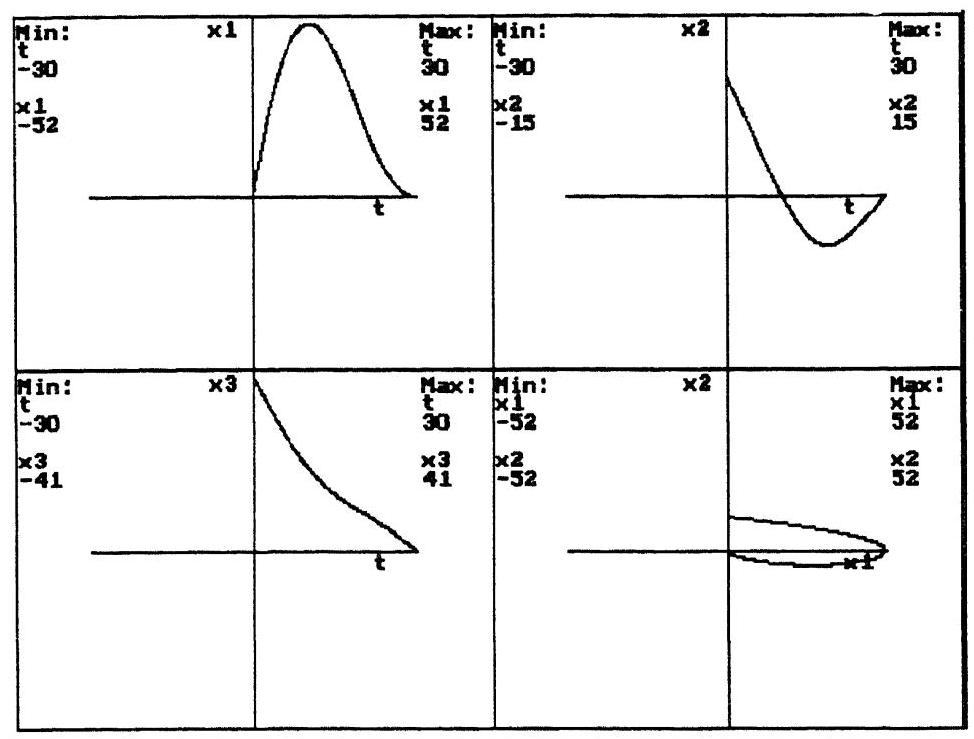
\includegraphics[max width=0.9\textwidth]{images/bo_d54811f7aajc73fuvcmg_26_271_86_974_739_0.jpg}
\end{center}
\hspace*{3em} 

Рис. 2

Задача Коши (3.24) принимает вид

\[
\left\{  \begin{array}{l} {\dot{x}}_{1} = {x}_{2}, \\  {\dot{x}}_{2} =  - 6{x}_{1}/{\theta }^{2} - 4{x}_{2}/\theta , \\  \dot{\theta } =  - \left( {{18}{x}_{1}^{2} + {18\theta }{x}_{1}{x}_{2} + 5{\theta }^{2}{x}_{2}^{2}}\right) /\left( {{12}{x}_{1}^{2} + {9\theta }{x}_{1}{x}_{2} + 2{\theta }^{2}{x}_{2}^{2}}\right) , \\  {x}_{1}\left( 0\right)  = {x}_{10}, \\  {x}_{2}\left( 0\right)  = {x}_{20}, \\  \theta \left( 0\right)  = {\theta }_{0}. \end{array}\right. \tag{3.25}
\]

Она имеет особенность в нуле. Результаты решения задачи (3.25), полученные с помощью программы КОШИ методом Фельберга с автоматическим выбором шага при 600 узлах для начальных данных

\[
{x}_{10} = 0,\;{x}_{20} = {10},\;{\theta }_{0} = {40},
\]

представлены на рис. 2. Вспомогательная переменная θ ≡ хз во избежание пе- реполнения в конце процесса вводилась в систему (3.25) в регуляризованном виде \({\left( \mu  + {\theta }^{2}\right) }^{1/2},\mu  = {10}^{-{10}}\) . При \(T = {29},{64}\) получено:

\[
{x}_{1}\left( T\right)  = 2,{718E} - {04},\;{x}_{2}\left( T\right)  =  - 1,{648E} - {02},\;\theta \left( T\right)  = 3,{301E} - {02},\;\left| u\right|  \leq  1
\]

Для объекта (3.14),(3.16) \(n = 2,{x}_{0} = \left( {0,{10}}\right) ,\left| u\right|  \leq  1\) ,время быстродействия равно \({10}\left( {1 + \sqrt{2}}\right)  \approx  {24},{14}.\)

При \(n > 2\) рассмотренная схема требует некоторой модификации.

3 аме ча н и е 3.5. Если в системе (3.25) третье уравнение взять в форме

\[
\dot{\theta } =  - 1,\;\theta \left( 0\right)  = {\theta }_{0},
\]

то \(\theta \left( t\right)  = {\theta }_{0} - t\) и первые два уравнения принимают вид

\[
\left\{  \begin{array}{l} {\dot{x}}_{1} = {x}_{2}, \\  {\dot{x}}_{2} =  - 6{x}_{1}/{\left( {\theta }_{0} - t\right) }^{2} - 4{x}_{2}/\left( {{\theta }_{0} - t}\right) ,\;0 \leq  t < {\theta }_{0}. \end{array}\right. \tag{3.26}
\]

Переход в (3.26) к новым переменным

\[
{y}_{1} = {x}_{1},\;{y}_{2} = \left( {{\theta }_{0} - t}\right) {x}_{2}
\]

свведением нового времени

\[
\tau  =  - \ln \left( {1 - t/{\theta }_{0}}\right) ,\;0 \leq  \tau  <  + \infty
\]

приводит к автономной системе

\[
\left\{  \begin{array}{l} d{y}_{1}/{d\tau } = {y}_{2}, \\  d{y}_{2}/{d\tau } =  - 6{y}_{1} - 5{y}_{2} \end{array}\right.
\]

с устойчивой матрицей, что позволяет получить в аналитической форме решение системы (3.26)

\[
{x}_{1}\left( t\right)  = {k}_{1}{\left( 1 - t/{\theta }_{0}\right) }^{2} + {k}_{2}{\left( 1 - t/{\theta }_{0}\right) }^{3},
\]

\[
{x}_{2}\left( t\right)  =  - \left( {2{k}_{1}\left( {1 - t/{\theta }_{0}}\right)  + 3{k}_{2}{\left( 1 - t/{\theta }_{0}\right) }^{2}}\right) /{\theta }_{0},
\]

\[
{k}_{1} = 3{x}_{10} + {\theta }_{0}{x}_{20},\;{k}_{2} =  - 2{x}_{10} - {\theta }_{0}{x}_{20}.
\]

Отсюда видно, что увеличение параметра \({\theta }_{0}\) приводит к уменьшению управляющего сигнала \(u = {\dot{x}}_{2}\) .

Графический пакет KOMU разработан на кафедре оптимального управления факультета вычислительной математики и кибернетики МГУ, его описание содер- жится в [37, 49]. Пакет KOIIИ предназначен для численного исследования систем обыкновенных дифференциальных уравнений на ПЭВМ IBM PC XT/AT. Широкий набор сервисных функций (встроенный графический редактор, многооконная гра- фика, двумерные и трехмерные проекции, масштабирование окна, вращение осей в трехмерном пространстве, калькулятор и другие возможности) делает пакет удоб- ным инструментом для научных и инженерных исследований. Пакет КОШИ можно также рекомендовать студентам вузов для использования в учебной и исследова- тельской работе.

Поступило в ноябре 1994 г.

\section*{ЛИТЕРАТУРА}

1. Понтрягин Л.C., Болтянский В.Г., Гамкрелидзе Р.В., Мищенко Е.Ф. Математическая тео- рия оптимальных процессов. М.: Наука, 1961.

2. Понтрягим Л.С. Избранные научные труды. М.: Наука, 1988. Т. 2.

3. Понтрягин Л.С. Принцип максимума в оптимальном управлении. М., 1990.

4. Гамкрелидзе P.B. Teopag оптимальных по быстродействию процессов в линейных системах // Изв. АН СССР. Сер. мат. 1958. Т. 22, № 4. С. 449-474.

5. Мищекко Е.Ф. Некоторые вопросы теории оптимального управления и преследования //Вто- рая летняя мат. шк. (Капивели, 1964). Киев, 1965. С. 93-124.

6. Болмянский В.Г. Математические методы оптимального управления. М., 1966.

7. Красовский Н.Н. Теория управления движением. М.: Hayka, 1968.

8. Neustadt L.W. Synthesizing time optimal control systems //J. Math. Anal. and Appl. 1960. Vol. 1. P. 484-493.

9. Eaton J.H. An iterative solution to time-optimal control //Ibid. 1962. Vol. 5, N 2. P. 329-344.

10. Пиеничный Б.Н. Численный метод расчета оптимального по быстродействию управления для линейных систем //Журн. вычисл. математики и мат. физики. 1964. № 1. С. 52-60.

11. Благодатски В.И. Линейная теория оптимального управления. М., 1978.

12. Белолипецкий А.А. Численный метод решения линейной задачи оптимального быстродействия сведением ее к задаче Коша //Журн. вычисл. математики и мат. физики. 1977. № 6. С. 1380- 1386.

13. Plant J.B., Athans M. An iterative technique fот the computation of time optimal controls //Proc. Third IFAC Congress. London. 1966. Pap. 13D. P. 1-10.

14. Федоренко Р.П. Приближенное решение задач оптимального управления. М., 1978.

15. Васильев Ф.П. Лекции по методам решения экстремальных задач. М., 1974.

16. Fujisawa T., Yasuda Y. An iterative procedure fот solving the time-optimal regulatот problem //J. SIAM Control. 1967. Vol. 5, N 4. P. 501-512.

17. Хайлов Е.Н. О приближенном отыскании моментов переключения //Проблемы современной математики в задачах физики и механики. М.: МФТИ, 1989. С. 136-139.

18. Kpācoвский H.H. Oб одном методе построения оптимальных траекторий //Мат. сб. 1961. № 2. С. 195-206.

19. Бабенко Л.B., Шаманский В.E. Численное построение оценок минимизируемого функционала в задачах на оптимальное быстродействие //Математическая физика. Киев, 1967. Вып. 2. С. 12-22.

20. Кун J.A., Пронозин Ю.Ф. К регуляризации метода Беллмана в задачах оптимального бы- стродействия // Докл. АН СССР. 1971. Т. 200, № 6. С. 1294-1297.

21. Тынянский Н.Т., Арутюнов А.В. К теории линейных процессов оптимального управления //Сообщ. АН ГССР. 1978. Т. 91, № 1. С. 29-31.

22. Сокол B.A., Тынянский Н.Т. Приблюженный метод решения линейной задачи оптимального быстродействия //Журн. вычисл. математики и мат. физики. 1980. № 2. С 277-288.

23. Киселев Ю. Н. Линейная теория быстродействия с возмущениями. М., 1986.

24. Киселев B Ю. Н. Методы решения гладкой линейной задачи быстродействия // Тр. МИАН СССР. 1988. Т. 185. С. 105-116.

25. Киселев B Ю. Н. Оптимальный синтез в гладкой линейной задаче быстродействия //Дифференц. уравнения. 1990. Т. 26, № 2. С. 232-237.

26. Киселев Ю.И. Быстросходящиеся алгоритмы решения линейной задачи быстродействия //Ка- бернетика. 1990. № 6. С. 47-57, 62.

27. Киселев Ю. Н., Орлов М.B. Численные алгоритмы линейных быстродействий //Журн. вы- числ. математики и мат. физики. 1991. № 12. С. 1763-1771.

28. Орлов М. В. Об одном численном алгоритме решения линейной задачи быстродействия //Co- временная математика в физико-технических задачах. М.: МФТИ, 1986. С. 67-76.

29. Орлов М.B. Линейная задача быстродействия. Численный алгоритм //Вестн. МГУ. Сер. 15, Вычисл. математика и кибернетика. 1986. № 4. С. 41-46.

30. Киселев Ю.И., Орлов М. В. Об одной схеме поиска оптимального решения линейной задачи быстродействия //Там же. 1986. № 2. С. 60-65.

31. Киселев Ю.H., Шимохина О.H. Асимптотика сглаживания в одной линейной задаче быстро- действия //Там же. 1984. № 4. С. 49-55.

32. Киселев Ю.И. Асимптотика времени быстродействия в линейной задаче управления маятни- ком при специальном возмущении (сглаживания) области управления //Там же. 1986. № 1. С. 57-61.

33. Аввакумов С.H. Асимптотика времени быстродействия в линейной задаче управления движе- нием маятника с двумерным управлением при специальном возмущении (слаживании) обла- сти управления //Вопросы вычислительной математики и программного обеспечения ЭВМ. M.: Изд-во МГУ, 1987.

34. Киселев Ю.И. Задача быстродействия с линейным терминальным множеством //Вестн. МГУ. Cep. 15, Вычисл. математика и кибернетика. 1991. № 4. С. 39-43.

35. Киселев B Ю. Н. Линейная задача быстродействия с гладкими множествами //III Всесоюз. ппк. Понтрягинские чтения "Оптимальное управление. Геометрия и анализ": Тез. докл. Кемерово, 1990. С. 147-148.

36. Рябов A.Ю., Орлов М. В. Графический пакет ТАЙМЕР для решения линейной задачи быстро- действия. М.: Центр "Диалог" в МГУ, 1991.

37. Орлов M.B., Рябов А.Ю. Графический пакет КОШИ для исследования систем дифференци- альных уравнений. М.: Центр "Диалог" в МГУ, 1992.

38. Лейтвейс К. Выпуклые множества. М., 1985.

39. Schneider R. Smooth approximation of convex bodies //Rend. Circ. mat. Palermo. 1984. Vol. 33. P. 436-440.

40. Рябов A.IO., Киселев IO.H., Орлов M.B. Пакет ТАЙМЕР — интегрированная среда для ис- следования линейной задачи быстродействия //Тез. докл. междунар. науч.-техн. конф. "Акту- альные проблемы фундаментальных наук". М.: МГТУ, 1991.

41. Kucene6 Ю.И. Асимптотическое решение задачи оптимального быстродействая для систем управления, близких к линейным //Докл. АН СССР. 1968. Т. 182, № 1. С. 31-34.

42. Фан Лянь-цень, Вань Чу-сень. Дискретный принцип максимума. М., 1967.

43. Болтянский В.Г. Оптимальное управление дискретными системами. М., 1973.

44. A йда-Заде К.Р. Исследование и численное решение конечно-разностных аппроксимаций задач управления с распределенными параметрами //Журн. вычисл. математики и мат. физики. 1989. № 3. С. 346-354.

45. Киселев 6 Ю. Н. Алгоритмы оптимизации дискретных линейных управляемых систем с гладкой областью управления //Тез. докл. Литовского мат. о-ва. Вильнюс, 1991. С. 106-107.

46. Киселев Ю.И., Шимохина О.И. Алгоритмы минимизации квадратичного терминального функ- пионала для дискретных линейных управляемых систем с гладкой областью управления и их приложения //Техническая кибернетика (Россия). 1993. № 4. С. 105-115.

47. Габасов Р., Кириллова Ф.М. Конструктивные методы оптимизации. Минск, 1984.

48. Коробов В.И. Общий подход к решению задачи синтеза ограниченных управлений в задаче управляемости //Мат. сб. 1979. Т. 109, № 4. С. 582-606.

49. Григоренко Н.Л., Орлов М. В., Рябов А.Ю. Программа КОШИ — интегрированная среда для исследования систем дифференциальных уравнений //Прикладное системное программное обеспечение СКП ЭВМ МГУ. М.: Изд-во МГУ, 1991. С. 76-96.
\end{document}